\section{Deep Discovery of Deep Options}
\label{ddco}
Since designing such hierarchical structures manually is infeasible in high-dimensional spaces, we need algorithms to discover them. Despite recent results in option discovery, some proposed techniques do not generalize well to multi-level hierarchies~\cite{kulkarni2016hierarchical, heess2016learning, baconHP16}, while others are inefficient for learning expressive representations~\cite{daniel2012hierarchical,lakshminarayananKKR16,hamidiTGF15,buiVW02}.

We introduce the \emph{Discovery of Deep Options (DDO)}, an algorithm for efficiently discovering deep hierarchies of deep options. DDO is a policy-gradient algorithm that discovers parametrized options from a set of demonstration trajectories (sequences of states and actions) provided either by a supervisor or by roll-outs of previously learned policies. These demonstrations need not be given by an optimal agent, but it is assumed that they are informative of the preferred actions to take in each visited state, and are not just random walks. DDO is an inference algorithm that applies to the \textbf{supervised demonstration setting}.

Given a set of trajectories, the algorithm discovers a fixed, predetermined number of options that are most likely to generate the observed trajectories. Since an option is represented by both a control policy and a termination condition, our algorithm simultaneously (1) infers option boundaries in demonstrations which segment trajectories into different control regimes, (2) infers the meta-control policy for selecting options as a mapping of segments to the option that likely generated them, and (3) learns a control policy for each option, which can be interpreted as a soft clustering where the centroids correspond to prototypical behaviors of the agent.

\subsection{Generative Model}
We generalize standard IL to hierarchical control, by introducing Hierarchical Behavioral Cloning (HBC) model. In HBC, the meta-control signals that form the hierarchy are unobservable, latent variables of the generative model, that must be inferred.

Consider a trajectory $\xi=(s_0,a_0,s_1,\ldots,s_T)$ that is generated by a two-level hierarchy. The low level implements a set $\C H$ of options $\lan \pi_h, \psi_h \ran_{h\in\C H}$. The high level implements a meta-control policy $\eta(h_t \given s_t)$ that repeatedly chooses an option $h_t\sim\eta(\cdot|s_t)$ given the current state, and runs it until termination. Our hierarchical generative model is:
\begin{algorithmic}
    \State Initialize $t\gets0$, $s_0 \sim p_0$, $b_0 \gets 1$
    \For{$t\gets0,\ldots,T-1$}
        \If{$b_t=1$}
            \State Draw $h_t \sim \eta(\cdot \given s_t)$
        \Else\Comment{$b_t=0$}
            \State Set $h_t \gets h_{t-1}$
        \EndIf
        \State Draw $a_t \sim \pi_{h_t}(\cdot \given s_t)$
	\State Draw $s_{t+1} \sim p(\cdot \given s_t, a_t)$
	\State Draw $b_{t+1} \sim \R{Ber}(\psi_{h_t}(s_{t+1}))$
    \EndFor
\end{algorithmic}


\subsection{Expectation-Gradient Inference Algorithm}
\slab{eg}
We denote by $\theta$ the vector of parameters for $\pi_h$, $\psi_h$ and $\eta$. For example, $\theta$ can be the weights and biases of a feed-forward network that computes these probabilities. This generic notation allows us the flexibility of a completely separate network for the meta-control policy and for each option, $\theta=(\theta_\eta,(\theta_h)_{h\in\C H})$, or the efficiency of sharing some of the parameters between options, similarly to a Universal Value Function Approximator~\cite{schaul2015universal}.

We want to find the $\theta\in\Theta$ that maximizes the log-likelihood assigned to a given dataset of trajectories. The likelihood of a trajectory depends on the latent sequence $\zeta = (b_0,h_0,b_1,h_1,\ldots,h_{T-1})$ of meta-actions and termination indicators, and in order to use a gradient-based optimization method we rewrite the gradient using the following \emph{EG-trick}:
\eq{
\nabla_\theta L[\theta;\xi] &= \nabla_\theta \log \p_\theta(\xi) = \frac 1 {\p_\theta(\xi)} \sum_{\zeta\in(\{0,1\}\times\C H)^T} \nabla_\theta \p_\theta(\zeta,\xi) \\
&= \sum_\zeta \frac {\p_\theta(\zeta,\xi)} {\p_\theta(\xi)} \nabla_\theta \log \p_\theta(\zeta,\xi) = \E_{\zeta|\xi;\theta}[\nabla_\theta \log \p_\theta(\zeta,\xi)],
}
which is the so-called \emph{Expectation-Gradient} method \cite{salakhutdinov2003optimization,mclachlan2007algorithm}. $\theta^-$ denotes the current parameter taken as fixed outside the gradient.

The generative model in the previous section implies the likelihood
\eq{
\p_\theta(\zeta,\xi) = p_0(s_0) \delta_{b_0=1}\eta(h_0 \given s_0) \prod_{t=1}^{T-1} \p_\theta(b_t, h_t \given h_{t-1}, s_t) \prod_{t=0}^{T-1} \pi_{h_t}(a_t \given s_t) p(s_{t+1} \given s_t, a_t) ,
}
with
\eq{
\p_\theta(b_t {=} 1, h_t \given h_{t-1}, s_t) &= \psi_{h_{t-1}}(s_t) \eta(h_t \given s_t) \\
\p_\theta(b_t {=} 0, h_t \given h_{t-1}, s_t) &= (1 - \psi_{h_{t-1}}(s_t)) \delta_{h_t = h_{t-1}}.
}
$\delta_{h_t = h_{t+1}}$ denotes the indicator that $h_t = h_{t+1}$.

Applying the EG-trick and ignoring the terms that do not depend on $\theta$, we can simplify the gradient to:
\eq{
\nabla_\theta L[\theta;\xi] = \E_{\zeta|\xi;\theta}\Bigg[\nabla_\theta \log \eta(h_0 \given s_0) + \sum_{t=1}^{T-1}\nabla_\theta \log \p_\theta(b_t, h_t \given h_{t-1}, s_t) + \sum_{t=0}^{T-1} \nabla_\theta \log \pi_{h_t}(a_t \given s_t) \Bigg].
}
%\eq{
%= {}& \mrlap{\sum_{h\in\C H} \p_\theta(h_0=h \given \xi) \nabla_\theta \log \eta_\theta(h \given s_0)} \\
%& + \mrlap{\sum_{t=0}^{T-1}\sum_{h\in\C H} \p_\theta(h_t=h \given \xi) \nabla_\theta \log \pi_{\theta;h}(a_t \given s_t) }\\
%& + \mrlap{\sum_{t=0}^{T-1}\sum_{h\in\C H} \p_\theta(h_t=h, b_t=1 \given \xi) \nabla_\theta \log \psi_{\theta;h}(s_{t+1})} \\
%& + \mrlap{\sum_{t=0}^{T-1}\sum_{h\in\C H} \p_\theta(h_t=h, b_t=0 \given \xi) \nabla_\theta \log (1 - \psi_{\theta;h}(s_{t+1}))} \\
%& + \mrlap{\sum_{t=0}^{T-1}\sum_{h\in\C H} \p_\theta(b_t=1, h_{t+1}=h \given \xi) \nabla_\theta \log \eta_\theta(h \given s_{t+1}).}
%}
The log-likelihood gradient can therefore be computed as the sum of the log-probability gradients of the various parameterized networks, weighed by the marginal posteriors
\eq{
u_t(h) &= \p_\theta(h_t {=} h \given \xi) \\
v_t(h) &= \p_\theta(b_t {=} 1, h_t {=} h \given \xi) \\
w_t(h) &= \p_\theta(h_t {=} h, b_{t+1} {=} 0 \given \xi).
}
In the Expectation-Gradient algorithm, the E-step computes $u$, $v$ and $w$, and the G-step updates the parameter with a gradient step, namely
\eq{
\nabla_\theta L[\theta;\xi] = \sum_{h\in\C H} \Biggl(& \sum_{t=0}^{T-1}\mrlap{ \Biggl(v_t(h) \nabla_\theta \log \eta(h \given s_t) +  u_t(h)\nabla_\theta \log \pi_h(a_t \given s_t)\Biggr)} \\ 
& + \sum_{t=0}^{T-2} \Biggl((u_t(h)-w_t(h)) \nabla_\theta \log \psi_h(s_{t+1}) + w_t(h) \nabla_\theta \log (1 - \psi_h(s_{t+1})) \Biggr)\Biggr).
}

These equations lead to the natural iterative algorithm. In each iteration, the marginal posteriors $u$, $v$ and $w$ can be computed with a forward-backward message-passing algorithm similar to Baum-Welch~\cite{baum1972equality}, with time complexity $O(|\C H|^2 T)$. Importantly, this algorithm can be performed without any knowledge of the state dynamics. The details of this computation are given in the supplementary material.
Then, the computed posteriors can be used in a gradient descent algorithm to update the parameters:
\eq{
\theta \gets \theta + \alpha \sum_i \nabla_\theta L[\theta;\xi_i].
}
This update can be made stochastic using a single trajectory, uniformly chosen from the demonstration dataset, to perform each update.

Intuitively, the algorithm attempts to jointly optimize three objectives:
\begin{itemize}
    \item Infer the option boundaries in which $b=1$ appears likely relative to $b=0$, as given by $(u-w)$ and $w$ respectively --- this segments the trajectory into regimes where we expect $h$ to persist and employ the same control law; in the G-step we reduce the cross-entropy loss between the unnormalized distribution $(w,u-w)$ and the termination indicator $\psi_h$;
    \item Infer the option selection after a switch, given by $v$; in the G-step we reduce the cross-entropy loss between that distribution, weighted by the probability of a switch, and the meta-control policy $\eta$; and
    \item Reduce the cross-entropy loss between the empirical action distribution, weighted by the probability for $h$, and the control policy $\pi_h$.
\end{itemize}
This can be interpreted as a form of soft clustering. 
The data points are one-hot representations of each $a_t$ in the space of distributions over actions.
Each time-step $t$ is assigned to option $h$ with probability $u_t(h)$, forming a soft clustering of data points.
The G-step directly minimizes the KL-divergence of the control policy $\pi_h$ from the weighted centroid of the corresponding cluster.

Let $\delta_{a_t}(a|s_t)=\delta_{a=a_t}$ be the degenerate ``empirical'' action distribution of step $t$.
The KL divergence of $\pi_h$ from the weighted centroid of the cluster corresponding to option $h$.

\subsubsection{Forward-Backward Algorithm}
\slab{forwardbackward}
Despite the exponential domain size of the latent variable $\zeta$, Expectation-Gradient for trajectories allows us to decompose the posterior $\p_\theta(\zeta \given \xi)$ and only concern ourselves with each marginal posterior separately. These marginal posteriors can be computed by a forward-backward dynamic programming algorithm, similar to Baum-Welch~\cite{?}.

Omitting the current parameter $\theta$ and trajectory $\xi$ from out notation, we start by computing the likelihood of a trajectory prefix
\eq{
\phi_t(h) = \p(s_0,a_0,\ldots,s_t,h_t=h),
}
using the forward recursion
\eq{
\phi_0(h) &= p_0(s_0) \eta(h \given s_0) \\
\phi_{t+1}(h') &= \sum_{h\in\C H} \nu_t(h) \pi_h(a_t \given s_t) p(s_{t+1} \given s_t, a_t) \p(h' \given h, s_{t+1}),
}
with
\eq{
\p(h' \given h, s_{t+1}) = \psi_h(s_{t+1}) \eta(h' \given s_{t+1}) + (1 - \psi_h(s_{t+1})) \delta_{h, h'}.
}
We similarly compute the likelihood of a trajectory suffix
\eq{
\omega_t(h) = \p(a_t,s_{t+1},\ldots,s_T \given s_t, h_t=h),
}
using the backward recursion
\eq{
\omega_T(h) &= 1 \\
\omega_t(h) &= \pi_h(a_t \given s_t) p(s_{t+1} \given s_t, a_t) \sum_{h'\in\C H} \p(h' \given h, s_{t+1}) \omega_{t+1}(h').
}

We can now compute our target likelihood using any $0\le t\le T$
\eq{
\p(\xi) = \sum_{h\in\C H} \p(\xi, h_t=h) = \sum_{h\in\C H} \phi_t(h) \omega_t(h).
}
The marginal posteriors are
\eq{
u_t(h) &= \frac{\phi_t(h) \omega_t(h)} {\p(\xi)} \\
v_t(h) &= \frac{\phi_t(h) \pi_h(a_t \given s_t) p(s_{t+1} \given s_t, a_t) \psi_h(s_{t+1}) \sum_{h'\in\C H} \eta(h' \given s_{t+1}) \omega_{t+1}(h')} {\p(\xi)} \\
w_t(h') &= \frac{\sum_{h\in\C H} \phi_t(h) \pi_h(a_t \given s_t) p(s_{t+1} \given s_t, a_t) \psi_h(s_{t+1}) \eta(h' \given s_{t+1}) \omega_{t+1}(h')} {\p(\xi)}.
}
Note that the constant $p_0(s_0) \prod_{t=0}^{T-1} p(s_{t+1} \given s_t, a_t)$ is cancelled out in these normalizations. This allows us to omit these terms during the forward-backward algorithm, which can thus be applied without any knowledge of the dynamics.


\subsubsection{Stochastic Variant}
We may collect a large number of trajectories making it difficult to scale the EG algorithm.
The expensive step in this algorithm is usually the forward-backward calculation, which is an $O(h^2T)$ operation.
To address this problem, we can apply a stochastic variant of the EG algorithm, which optimizes a single trajectory for each iterate:
\begin{itemize}
    \item \textbf{E-Step: } Draw a trajectory $i$ at random, calculate $q_i(t,h)$, and $b_i(t,h)$ with the forward-backward algorithm.
   \item \textbf{G-Step: } Update the parameters of the policies and the termination conditions:
    \[
\theta_h^{(j+1)} \leftarrow \theta_i^{(j)} - \alpha  \sum_{t=1}^{T} w_i(h,t) \nabla_\theta \log \pi_\theta(a_t \given s_t).
\]
\[
\mu_h^{(j+1)} \leftarrow \mu_i^{(j)} - \alpha \sum_{t=1}^{T} q_i(h,t) \nabla_\mu \log \rho_\mu(\perp \given s_t).
\]
\end{itemize}


\subsubsection{Deeper Hierarchies}
Our ultimate goal is to use the algorithm presented here to discover a multi-level hierarchical structure --- the key insight being that the problem is recursive in nature.
A $D$-level hierarchy can be viewed as a 2-level hierarchy, in which the ``high level'' has a $(D-1)$-level hierarchical structure. 
The challenge is the coupling between the levels; namely, the value of a set of options is determined by its usefulness for meta-control~\cite{foxMT16}, while the value of a meta-control policy depends on which options are available. This potentially leads to an exponential growth in the size of the latent variables required for inference.
The available data may be insufficient to learn a policy so expressive.

We can avoid this problem by using a simplified parametrization for the intermediate meta-control policy $\eta_d$ used when discovering level-$d$ options. In the extreme, we can fix a uniform meta-control policy that chooses each option with probability $\nicefrac 1 {|\C H_d|}$. Discovery of the entire hierarchy can now proceed recursively from the lowest level upward: level-$d$ options can invoke already-discovered lower-level options; and are discovered in the context of a simplified level-$d$ meta-control policy, decoupled from higher-level complexity.
One of the contributions of this work is to demonstrate that, perhaps counter-intuitively, this assumption does not sacrifice too much during option discovery.
An informative meta-control policy would serve as a prior on the assignment of demonstration segments to the options that generated them, but with sufficient data this assignment can also be inferred from the low-level model, purely based on the likelihood of each segment to be generated by each option.

We use the following algorithm to iteratively discover a hierarchy of $D$ levels, each level $d$ consisting of $k_d$ options:
\begin{algorithmic}
    \For{$d=1,\ldots,D-1$}
        \State Initialize a set of options $\C H_d=\{h_{d,1},\ldots,h_{d,k_d}\}$
        \State \alg: train options $\lan \pi_h, \psi_h \ran_{h\in\C H_d}$ with $\eta_d$ fixed
        \State Augment action space $\C A \gets \C A \cup \C H_d$
    \EndFor
    \State Use RL algorithm to train high-level policy
\end{algorithmic}

%To illustrate this point, some of our experiments model the meta-control policy as uniformly choosing each option with probability $\nicefrac 1 {|\C H|}$, only at the option discovery stage.

First, we approximate the high-level policy $\psi$, which selects policies based on the current state, with a i.i.d selection of policies based on only the previous primitive:
\[
\psi \sim \mathbf{P}(h' \given h)
\]
This approximation is so that we do not have to simultaneously learn parameters for the high-level policy, while trying to optimize for the parameters of the policies and termination conditions.
Next, if we collect trajectories from multiple high-level policies, there may not exist a single high-level policy that can capture all of the trajectories.
The approximation allows us to make the fewest assumptions about the structure of this policy.

Using an approximation that $\psi^*$ is a state-independent uniform distribution and sampled i.i.d, this paper will show the we can apply an algorithm similar to typical imitation learning approaches that recovers the most likely parameters to estimate $\pi^*_{1},...,\pi^*_{k}$ and $\{\rho^*_{1},...,\rho^*_{k}\}$. The basic idea is to define a probability that the current $(s_t,a_t)$ tuple is generated by the particular primitive $h$:
\[
w(h,t) = \mathbf{P}[h \given (s_t, a_t), \tau_{0<t}],
\]
and given that the current selected primitive is $h$ probability that the current time-step is termination:
\[
q(h,t) = \mathbf{P}[\perp \given (s_t, a_t), \tau_{0<t}, h].
\]
Given these probabilities, we can define an Expectation-Gradient descent over the parameter vector $\theta$
\eq{
\theta \gets \theta + \alpha \nabla_\theta L[\theta;\xi].
}


\subsubsection{Cross-Validation For Parameter Tuning}
The number of options $k$ is a crucial hyper-parameter of the algorithm.
In simulation experiments, one can roll out the learned hierarchy online and tune the hierarchy based on task success.
Such tuning is infeasible on a real robot as it would require many executions of the learned policy.
We explored whether it is possible to tune the number of options offline.
\alg is based on a maximum-likelihood formulation, which describes the likelihood that the observed demonstrations are generated by a hierarchy parametrized by $\theta$.
However, the model expressiveness is strictly increasing in $k$, causing the optimal training likelihood to increase even beyond the point where the model overfits to the demonstrations and fails to generalize to unseen states.

This likelihood is a proxy for task success.
Therefore, we tune $k$ in a way that maximizes the likelihood.
However, we sometimes encounter a problem similar to over-fitting.
Increasing $k$ actually changes expressiveness the hierarchy, as with more options it can fit to more complicated behaviors.
This means that the tuned parameters may not generalize.

We therefore adopt a cross-validation technique that holds out 10\% of the demonstration trajectories for each of $10$ folds, trains on the remaining data, and validates the trained model on the held out data.
We select the value of $k$ that achieves the highest average log-likelihood over the $10$ folds, suggesting that training such a hierarchical model generalizes well.
We train the final policy over the entire data.
This means the tuned parameter must work well on a hold out set.
We find empirically that the cross-validated log-likelihood serves as a good proxy to actual task performance.

\subsubsection{Vector Quantization For Initialization}
One challenge with DDO is initialization.
When real perceptual data is used, if all of the low-level policies initialize randomly the forward-backward estimates needed for the Expectation-Gradient will be poorly conditioned where there is an extremely low likelihood assigned to any particular observation.
The EG algorithm relies on a segment-cluster-imitate loop, where initial policy guesses are used to segment the data based on which policy best explains the given time-step, then the segments are clustered, and the policies are updated.
In a continuous control space, a randomly initialized policy may not explain any of the observed data well.
This means the small differences in initialization can lead to large changes in the learned hierarchy.

We found that a necessary pre-processing step was a variant of vector quantization, originally proposed for problems in speech recognition. 
We first cluster the state observations using a \textsf{k-means} clustering and train $k$ behavioral cloning policies for each of the clusters.
We use these $k$ policies as the initialization for the EG iterations.
Unlike the random initialization, this means that the initial low level policies will demonstrate some preference for actions in different parts of the state-space.
We set $k$ to be the same as the $k$ set for the number of options, and use the same optimization parameters.

\subsection{Experiments: Imitation}
In the first set of experiments, we evaluate DDO in its ability to represent hierarchical control policies. We find that the hierarchical representation is often easier to learn.

\subsubsection{Box2D Simulation: 2D Surface Pushing with Friction and Gravity}
In the first experiment, we simulate a 3-link robot arm in Box2D (Figure \ref{fig:b2dexp}). This arm consists of three links of lengths 5 units, 5 units, and 3 units, connected by ideal revolute joints. The arm is controlled by setting the values of the joint angular velocities $\dot{\phi}_1, \dot{\phi}_2, \dot{\phi}_3$. In the environment, there is a box that lies on a flat surface with uniform friction. The objective is to push this box without toppling it until it rests in a randomly chosen goal position. After this goal state is reached, the goal position is regenerated randomly.
The task is for the robot to push the box to as many goals as possible in 2000 time-steps.
Our algorithmic supervisor runs the RRT Connect motion planner of the Open Motion Planning Library, \textsf{ompl}, at each time-step planning to reach the goal. 
Due to the geometry of the configuration space and the task, there are two classes of trajectories that are generated, when the goal is to the left or right of the arm. 

\vspace{0.25em}\noindent \textbf{Algorithmic Supervisor: } Our algorithmic supervisor runs an RRT Connect motion planner (from the Open Motion Planning Library \textsf{ompl}) at each time-step planning till the goal. The motion planning algorithm contains a single important hyper-parameter which is the maximum length of branches to add to the tree. We set this at 0.1 units (for a 20 x 20 unit space).

\begin{figure}[t]
    \centering
    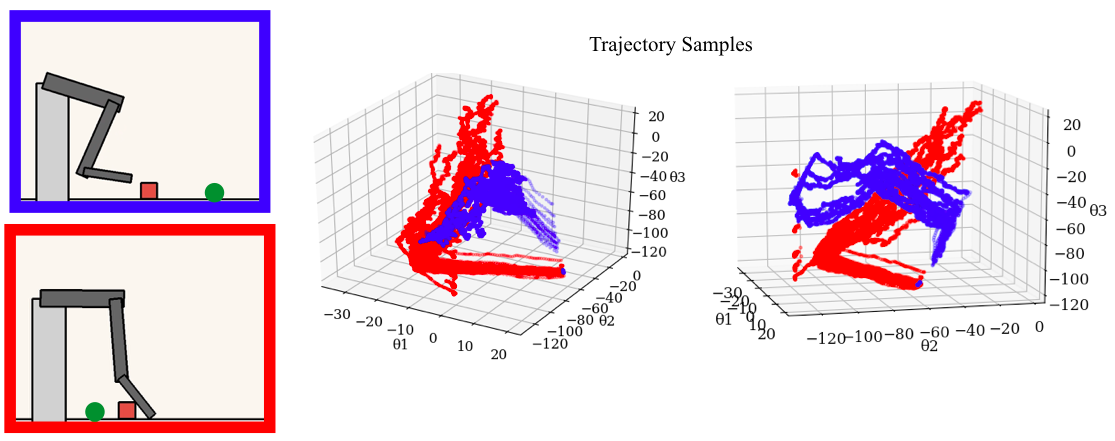
\includegraphics[width=\textwidth]{ddco-experiments/c-space.png}
    \caption{Due to the collision and contact constraints of the 2D Surface Pushing task, it leads to two geometrically distinct pushing skills, backhand and forehand, for goals on the left and on the right. Right: 50 sampled trajectories from a motion-planning supervisor. \label{fig:b2dcspace}}
\end{figure}

\vspace{0.25em}\noindent \textbf{Task Geometry: } We designed this experiment to illustrate how options can lead to more concise representations since they can specialize in different regions of the state-spaces.
Due to the geometry of the configuration space and the task, there are two classes of trajectories that are generated, when the goal is to the left or right of the arm.
The 50 sampled trajectories plotted in joint angle space in Figure \ref{fig:b2dcspace} are clearly separated into two distinct skills, backhand and forehand. 
Furthermore, these skills can be implemented by a locally affine policies in the joint angle space.

\vspace{0.25em}\noindent\textbf{Observing Positions and Orientations: } First, we consider the case where we observe the full low-dimensional state of the system: three joint angles, the box's position and orientation, and the position of the goal state. 
We compare our hierarchical policies with two flat, non-hierarchical policies. One baseline policy we consider is an under-parametrized linear policy which is not expressive enough to approximate the supervisor policy well. The other baseline policy is a multi-layer perceptron (MLP) policy.
We train each of these policies via Behavior Cloning (BC), i.e. by maximizing the likelihood each gives to the set of demonstrations.
As expected, the flat linear policy is unsuccessful at the task for any number of observed demonstrations (Figure \ref{fig:b2dexp1-1} Top-A). The MLP policy, on the other hand, can achieve the maximum reward when trained on 60 demonstrations or more. 

We apply \alg and learn two 2-level hierarchical policies, one with linear low-level options, and the other with MLP low-level options of the same architecture used for the flat policy. 
In both cases, the termination conditions are parametrized by a logistic regression from the state to the termination probability, and the high-level policy is a logistic regression from the state to an option selection.
For the linear hierarchy we set \alg to discover 5 options, and for the MLP hierarchy we discover 2 options.
The MLP hierarchical policy can achieve the maximum reward with  30 demonstrations, and is therefore 2x more sample-efficient than its flat counterpart (Figure \ref{fig:b2dexp1-1} Top A).
The experimental details are described below:

\vspace{0.25em}\noindent \textbf{Multi-Layer Perceptron Flat Policy: } One of the baseline policies is a multi-layer perceptron (MLP) policy which has a single ReLU hidden layer of 64 nodes.
This policy is implemented in Tensorflow and is trained with an ADAM optimizer with learning rate $1e-5$.

\vspace{0.25em}\noindent \textbf{\alg Policy 1: } In the first policy trained by \alg, we have a logistic regression meta-policy that selects from one of $k$ linear sub-policies. The linear sub-policies execute until a termination condition determined again by a logistic regression. This policy is implemented in Tensorflow and is trained with an ADAM optimizer with learning rate $1e-5$. For the linear hierarchy, we set \alg to discover 5 options, which is tuned using the cross-validation method described in the paper.

\vspace{0.25em}\noindent \textbf{\alg Policy 2: } In the second policy trained by \alg, we have a logistic regression meta-policy that selects from one of $k$ multi-layer perceptron sub-policies. 
As with the flat policy, it has a single ReLU hidden layer of 64 nodes.
The MLP sub-policies execute until a termination condition determined again by a logistic regression. This policy is implemented in Tensorflow and is trained with an ADAM optimizer with learning rate $1e-5$. For the MLP hierarchy, we set \alg to discover 2 options, which is tuned using the cross-validation method described in the paper.


\begin{figure}[t]\vspace{-2em}
    \centering
    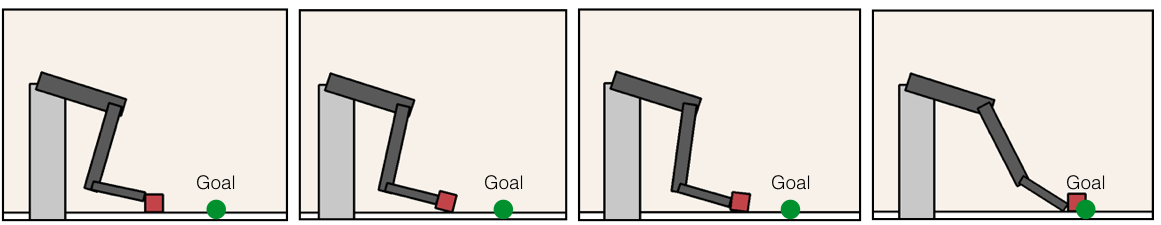
\includegraphics[width=0.8\textwidth]{ddco-experiments/2d-sp-friction.png}
    \caption{A 3-link robot arm has to push a box along a surface with friction to a randomly chosen goal state to the box's left or right without toppling it. Due to the collision and contact constraints of this task, it has two geometrically distinct pushing skills, backhand and forehand, for goals on the left and on the right. \label{fig:b2dexp}} 
\end{figure}

\begin{figure}[t]
    \centering
    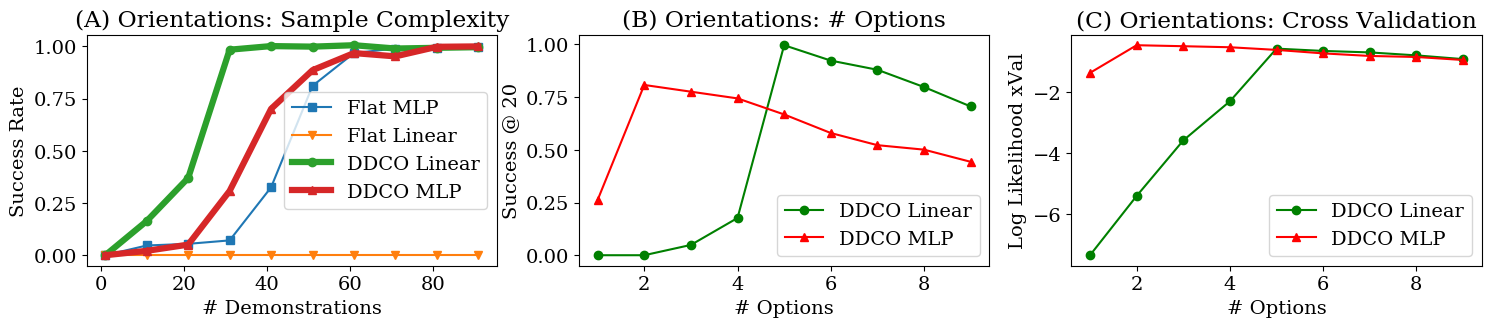
\includegraphics[width=0.8\textwidth]{ddco-experiments/exp1-1.png}
    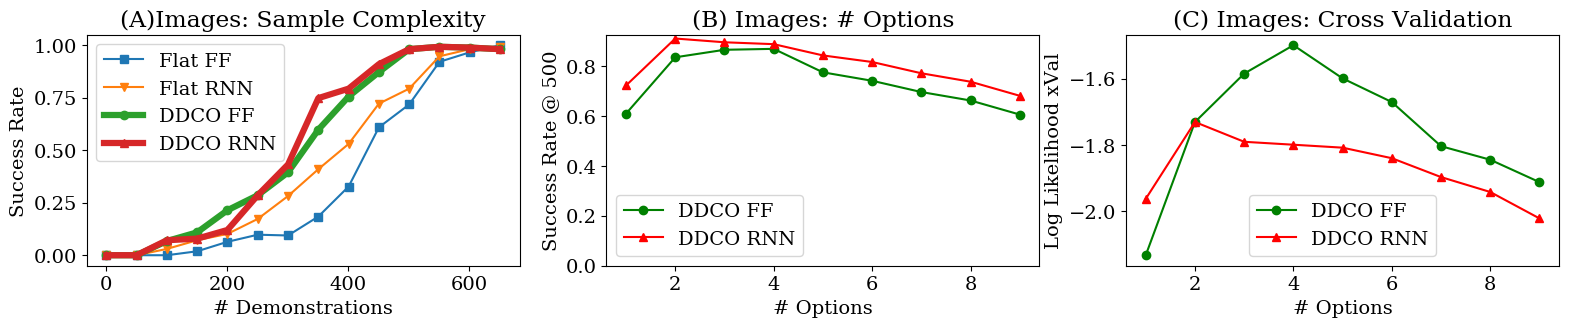
\includegraphics[width=0.8\textwidth]{ddco-experiments/exp1-2.png}
    \caption{2D Surface Pushing from low-dimensional observations and image observations. (A) The sample complexity of different policy representations, (B) The success rate for different numbers of discovered options, (C) The peak in the reward correlates over the number of options with the 10-fold cross-validated log-likelihood. \label{fig:b2dexp1-1}}
\end{figure}



We also vary the number of options discovered by \alg, and plot the reward obtained by the resulting policy (Figure \ref{fig:b2dexp1-1} Top-B). While the performance is certainly sensitive to the number of options, we find that the benefit of having sufficiently many options is only diminished gradually with each additional option beyond the optimum. Importantly, the peak in the cross-validated log-likelihood corresponds to the number of options that achieves the maximum reward (Figure \ref{fig:b2dexp1-1} Top-C). This allows us to use cross-validation to select the number of options without having to evaluate the policy by rolling it out in the environment.



\vspace{0.25em}\noindent\textbf{Observing Images: } Next, we consider the case where the sensor inputs are 640x480 images of the scene. The low-dimensional state is still fully observable in these images, however these features are not observed explicitly, and must be extracted by the control policy. We consider two neural network architectures to represent the policy: a convolutional layer followed by either a fully connected layer or an LSTM, respectively forming a feed-forward (FF) network and a recurrent network (RNN).
We use these architectures both for flat policies and for low-level options in hierarchical policies.
For the hierarchical policies, as in the previous experiment, we consider a high-level policy that only selects options.
For the FF policy we discover 4 options, and for the RNN policy we discover 2 options.
The experimental details are listed below. 
 
 \vspace{0.25em}\noindent \textbf{\alg FF Policy: } First, we consider a neural network with a convolutional layer with 64 5x5 filters followed by a fully connected layer forming a feed-forward (FF) network. The high-level model only selects options and is parametrized by the same general architecture with an additional softmax layer after the fully connected layer. This means that the meta-control policy is a two-layer convolutional network whose output is a softmax categorical distribution over options. This policy is implemented in Tensorflow and is trained with an ADAM optimizer with learning rate $1e-5$.
 We used $k=2$ options for the FF policy.
 
 \vspace{0.25em}\noindent \textbf{\alg RNN Policy: } Next, we consider a neural network with a convolutional layer with 64 5x5 filters followed by an LSTM layer forming  a recurrent network (RNN). The high-level model only selects options and is parametrized by the same general architecture with an additional softmax layer after the LSTM. This policy is implemented in Tensorflow and is trained with a Momentum optimizer with learning rate $1e-4$ and momentum $4e-3$.
  We used $k=4$ options for the RNN policy.
  
  \begin{figure}[t]
    \centering
    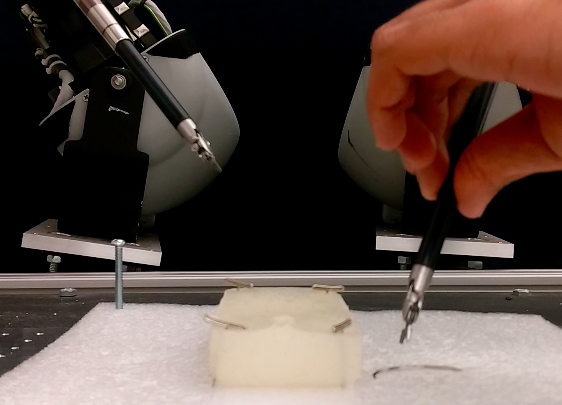
\includegraphics[width=0.48\textwidth]{ddco-experiments/demo-1.png}
    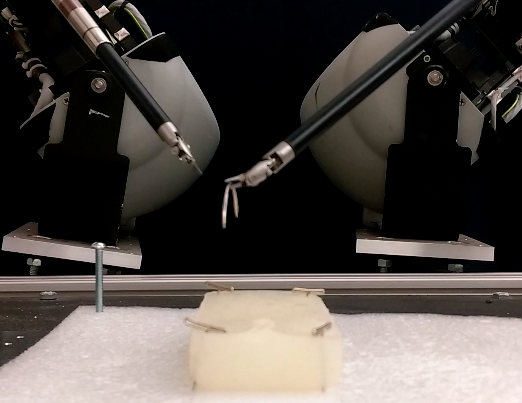
\includegraphics[width=0.455\textwidth]{ddco-experiments/demo-2.png}
    \caption{To collect demonstrations, we programmed an initial open-loop control policy. We observed the policy execute and interrupted the robot via keyboard input when adjustment was needed.  \label{fig:demo}}
\end{figure}
 


\begin{figure}[t]\vspace{-2em}
    \centering
    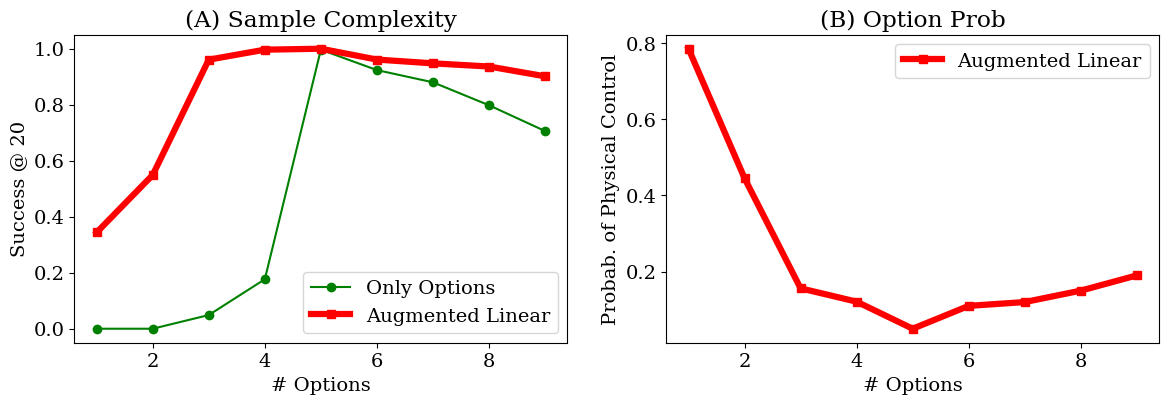
\includegraphics[width=0.8\textwidth]{ddco-experiments/exp1-3.png}
    \caption{ (A) The sample complexity of augmented v.s. option-only high-level control spaces. (B) The fraction of high-level selections that are of physical control. The frequency of selecting a physical control first decreases with the number of options, then increases as options overfit. \label{fig:b2dexp1-3}}
\end{figure}


The hierarchical policies require 30\% fewer demonstrations than the flat policies to achieve the maximum reward (Figure \ref{fig:b2dexp1-1} Bottom-A).
Figure \ref{fig:b2dexp1-1} Bottom-B and C show how the success rate and cross-validated log-likelihood vary with the number of options.
As for the low-dimensional inputs, the success rate curve is correlated with the cross-validated log-likelihood.
We can rely on this to select the number of options offline without rolling out the learned hierarchical policy.


\vspace{0.25em}\noindent\textbf{Control Space Augmentation (Kinematic): } 
We test two different architectures for the output layer of the high-level policy: either a softmax categorical distribution selecting an option, or the hybrid categorial--continuous distribution output described in~\sref{hybrid}.
The low-level policies are linear.

Figure \ref{fig:b2dexp1-3} describes the empirical estimation, through policy rollouts, of the success rate as a function of the number of options, and of the fraction of time that the high-level policy applies physical control.
When the options are too few to provide skills that are useful throughout the state space, physical controls can be selected instead to compensate in states where no option would perform well. This is indicated by physical control being selected with greater frequency. As more options allow a better coverage of the state space, the high-level policy selects physical controls less often, allowing it to generalize better by focusing on correct option selection. With too many discovered options, each option is trained from less data on average, making some options overfit and become less useful to the high-level policy.

\vspace{0.25em}\noindent\textbf{Control Space Augmentation (Images): }  We ran the same experiment but on the image state-space instead of the low dimensional state.
The sensor inputs are 640x480 images of the scene and the task is the Box2D pushing task.
Figure \ref{fig:augimages} describes the empirical estimation, through policy rollouts, of the success rate as a function of the number of options, and of the fraction of time that the high-level policy applies physical control.
When the options are too few to provide skills that are useful throughout the state space, physical controls can be selected instead to compensate in states where no option would perform well. 

\begin{figure} [t]
\centering
    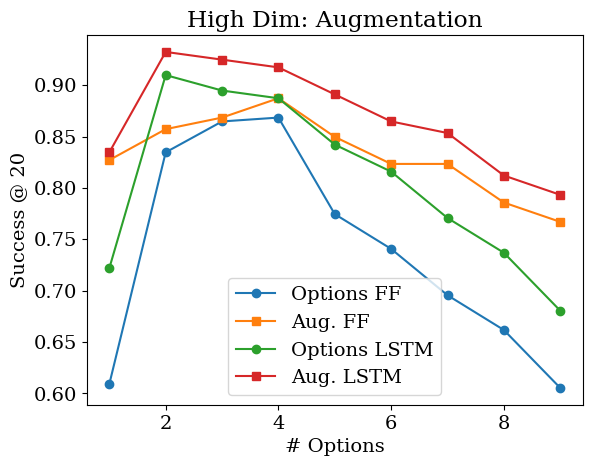
\includegraphics[width=0.4\textwidth]{ddco-experiments/exp7-1.png}
    \caption{Augmenting the action space instead of selecting only options with the meta-policy leads attenuates the losses when selecting too few or too many options. \label{fig:augimages}}
\end{figure}



\subsubsection{Physical Experiment 1: Needle Insertion}
We consider a needle orientation and insertion task on the da Vinci Research Kit (DVRK) surgical robot (Figure \ref{fig:dvrkexp3}). In this task, the robot must grasp a surgical needle, reorient it in parallel to a tissue phantom, and insert the needle into the tissue phantom.
The task is successful if the needle is inserted into a 1cm diameter target region on the phantom. Small changes in the needle's initial orientation can lead to large changes in the in-gripper pose of the needle due to deflection. 
The state is the current 6-DoF pose of the robot gripper, and algorithmically extracted visual features that describe the estimated pose of the needle.
These features are derived from an image segmentation that masks the needle from the background and fits an ellipsoid to the resulting pixels. 
The principal axis of this 2D ellipsoid is a proxy for the pose of the needle.
The task runs for a fixed 15 time-steps, and the policy must set the joint angles of the robot at each time-step.

\begin{figure}
    \centering
    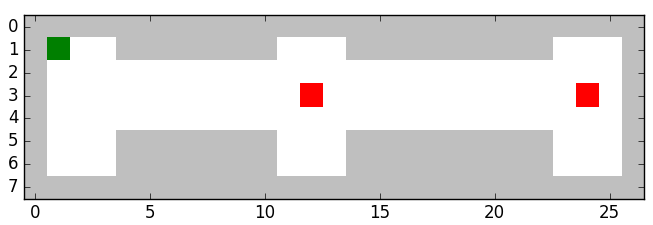
\includegraphics[width=0.8\textwidth]{ddco-experiments/exp3.png}
    \caption{A needle orienting and insertion task. The robot must grasp a surgical needle, reorient it in parallel to a tissue phantom, and insert the needle.   \label{fig:dvrkexp3}}
\end{figure}

The needle's deflection coupled with the inaccurate kinematics of the DVRK make it challenging to plan trajectories to insert the needle properly.
A visual servoing policy needs to be trained that can both grasp the needle in the correct position, as well as reorient the gripper in the correct direction after grasping.
To collect demonstrations, we programmed an initial open-loop control policy, interrupted the robot via keyboard input when adjustment was needed, and kinesthetically adjusted the pose of the gripper. 
We collected 100 such demonstrations.

 We evaluated the following alternatives: (1) a single flat MLP policy with continuous output, (2) a flat policy consisting of 15 distinct MLP networks, one for each time-step, (3) a hierarchical policy with 5 options trained with \alg. We considered a hierarchy where the high-level policy is a MLP with a softmax output that selects the appropriate option, and each option is parametrized by a distinct MLP with continuous outputs.
 \alg learns 5 options, two of which roughly correspond to the visual servoing for grasping and lifting the needle, and the other three handle three different types of reorientation.
 For 100 demonstrations, the hierarchical policy learned with \alg has a 45\%  higher log-likelihood measured in cross-validation than the flat policy, and a 24\% higher log-likelihood than the per-timestep policy. 
 The experimental details are described below:
 
\vspace{0.5em} \noindent \textbf{Task Description: } The robot must grasp a 1mm diameter surgical needle, re-orient it parallel to a tissue phantom, and insert the needle into a tissue phantom.
The task is successful if the needle is inserted into a 1 cm diameter target region on the phantom.
In this task, the state-space is the current 6-DoF pose of the robot gripper and visual features that describe the estimated pose of the needle.
These features are derived from an image segmentation that masks the needle from the background and fits an ellipsoid to the resulting pixels. 
The principal axis of this 2D ellipsoid is a proxy for the pose of the needle.
The task runs for a fixed 15 time-steps and the policy must set the joint angles of the robot at each time-step.

\vspace{0.5em} \noindent \textbf{Robot Parameters: } The challenge is that the curved needle is sensitive to the way that it is grasped. Small changes in the needle's initial orientation can lead to large changes to the in-gripper pose of the needle due to deflection.
This deflection coupled with the inaccurate kinematics of the DVRK leads to very different trajectories to insert the needle properly.

The robotic setup includes a stereo endoscope camera located 650 mm above the 10cm x 10 cm workspace.
After registration, the dvrk has an RMSE kinematic error of 3.3 mm, and for reference, a gripper width of 1 cm.
In some regions of the state-space this error is even higher, with a 75\% percentile error of 4.7 mm.
The learning in this task couples a visual servoing policy to grasp the needle with the decision of which direction to orient the gripper after grasping.

\vspace{0.5em} \noindent \textbf{Demonstration Protocol: }
To collect demonstrations, we programmed an initial open-loop control policy. This policy traced out the basic desired robot motion avoiding collisions and respecting joint limits, and grasping at where it believed the needle was and an open-loop strategy to pin the needle in the phantom.
This was implemented by 15 joint angle way points which were interpolated by a motion planner.
We observed the policy execute and interrupted the robot via keyboard input when adjustment was needed.
This interruption triggered a clutching mechanism and we could 
kinesthetically adjusted the joints of the robot and pose of the gripper (but not the open-close state).
The adjustment was recorded as a delta in joint angle space which was propagated through the rest of the trajectory.
We collected 100 such demonstrations and images of these adjustements are visualized in image (Figure \ref{fig:demo}).

\begin{figure}
    \centering
    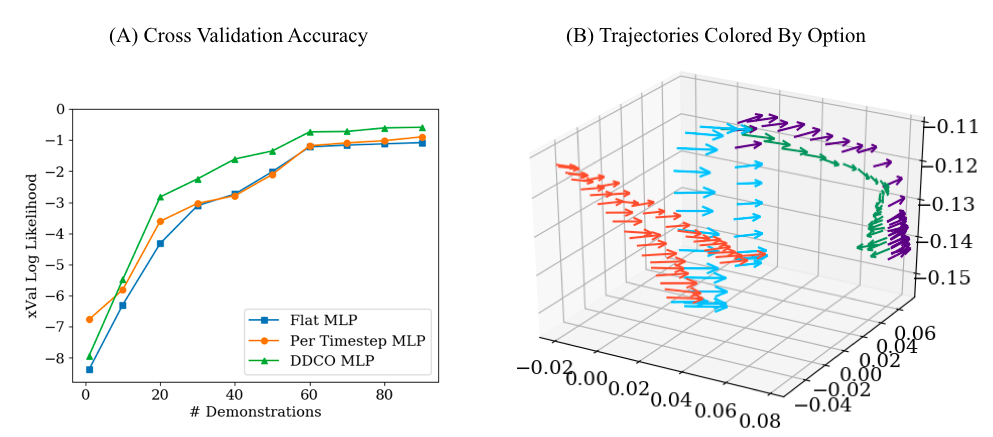
\includegraphics[width=\textwidth]{ddco-experiments/exp-5-1-1.png}
    \caption{(A) We plot the cross validation likelihood of the different methods as a function of the number of demonstrations. (B) We visualize two representative trajectories (position and gripper orientation) color coded by the most likely option applied at that timestep. We find that the two trajectories have the same first two options but then differ in the final step due to the re-orientation of the gripper before insertion.  \label{fig:dvrkexp1}}
\end{figure}


\vspace{0.25em} \noindent \textbf{Learning the Parameters: } Figure \ref{fig:dvrkexp1}A plots the cross-validation log-likelihood as a function of the number of demonstrations.
We find that the hierarchical model has a higher likelihood than the alternatives---meaning that it more accurately explains the observed data and generalizes better to held out data.
At some points, the relative difference is over 30\%.
It, additionally, provides some interpretability to the learned policy.
Figure \ref{fig:dvrkexp1}B visualizes two representative trajectories.
We color code the trajectory based on the option active at each state (estimated by \alg).
The algorithm separates each trajectory into 3 segments: needle grasping, needle lifting, and needle orienting.
The two trajectories have the same first two options but differ in the orientation step.
One of the trajectories has to rotate in a different direction to orient the needle before insertion.


\vspace{0.25em} \noindent \textbf{Flat Policy: } One of the baseline policies is a multi-layer perceptron (MLP) policy which has a single ReLU hidden layer of 64 nodes.
This policy is implemented in Tensorflow and is trained with an ADAM optimizer with learning rate $1e-5$.

\vspace{0.25em} \noindent \textbf{Per-Timestep Policy: } Next, we consider a degenerate case of options where each policy executes for a single-timestep. We train 15 distinct multi-layer perceptron (MLP) policies each of which has a single ReLU hidden layer of 64 nodes.
Thes policies are implemented in Tensorflow and are trained with an ADAM optimizer with learning rate $1e-5$.

\vspace{0.25em} \noindent \textbf{\alg Policy: } \alg trains a hierarchical policy with 5 options. We considered a hierarchy where the meta policy is a multilayer perceptron with a softmax output that selects the appropriate option, and the options are parametrized by another multilayer perceptron with continuous outputs. Each of the MLP policies has a single ReLU hidden layer of 64 nodes.
Thes policies are implemented in Tensorflow and are trained with an ADAM optimizer with learning rate $1e-5$.


\vspace{0.25em} \noindent \textbf{Execution: } 
For each of the methods, we execute ten trials and report the success rate (successfully grasped and inserted the needle in the target region), and the accuracy.
The results are described in aggregate in the table below:

\begin{table}[ht!]\footnotesize
\centering
\label{my-label}
\begin{tabular}{l|l|l|l|l|}
             & Overall Success & Grasp Success & Insertion Success & Insertion Accuracy \\
             \hline
Open Loop    & 2/10   & 2/10  & 0/0 & $7 \pm 1$ mm                  \\
Behavioral Cloning & 3/10 & 6/10  & 3/6 &   $6 \pm 2$ mm     \\
Per Timestep & 6/10  & 7/10  & 6/7 &   $5 \pm 1$ mm \\ 
\alg & 8/10 & 10/10 & 8/10 &  $5 \pm 2$ mm  \\
\end{tabular}
\end{table}

\begin{figure}
    \centering
    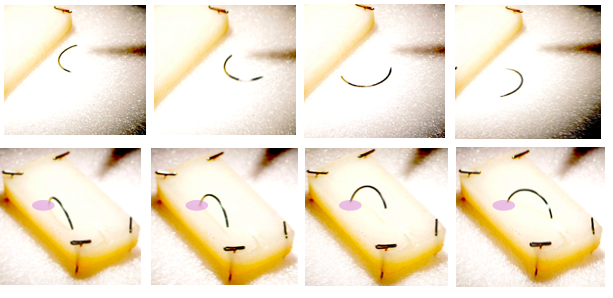
\includegraphics[width=0.8\textwidth]{ddco-experiments/exp3-1.png}
    \caption{Illustration of the needle orientation and insertion task. Above are images illustrating the variance in the initial state, below are corresponding final states after executing \alg.  \label{fig:dvrkexp3-1}}
\end{figure}


\begin{figure}
    \centering
    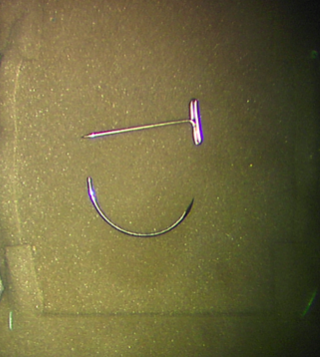
\includegraphics[width=0.25\textwidth]{ddco-experiments/image.png}
    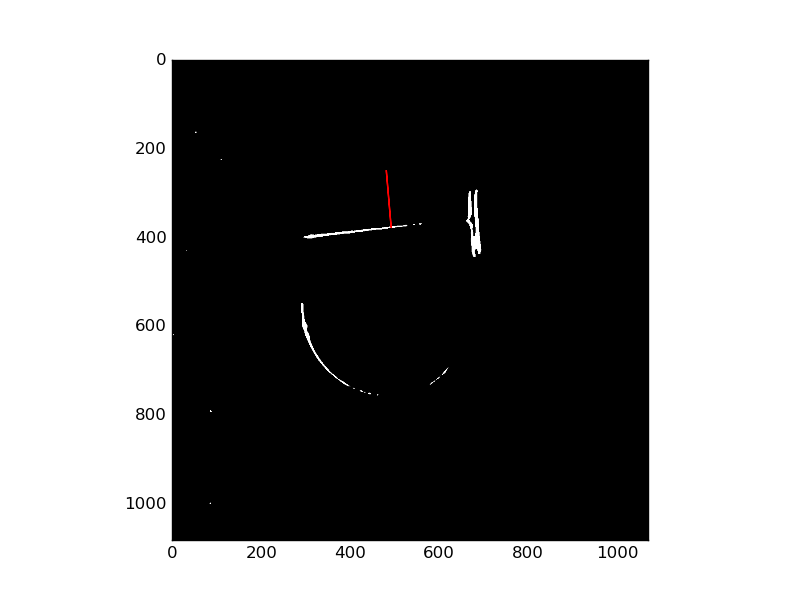
\includegraphics[width=0.4\textwidth]{ddco-experiments/binary-mask.png}
    \caption{The endoscope image and a corresponding binary mask with a selected grasp. The arrow corresponds to the orientation of the gripper along the grasp axis.  \label{fig:dvrkim}}
\end{figure}

 

We ran preliminary trials to confirm that the trained options can be executed on the robot.
For each of the methods, we report the success rate in 10 trials, i.e. the fraction of trials in which the needle was successfully grasped and inserted in the target region. %We also report the insertion accuracy.
All of the techniques had comparable accuracy in trials where they successfully grasped and inserted the needle into the 1cm diameter target region.
The algorithmic open-loop policy only succeeded 2/10 times.
Surprisingly, Behavior Cloning (BC) did not do much better than the open-loop policy, succeeding only 3/10 times.
Per-timestep BC was far more successful (6/10).
Finally, the hierarchical policy learned with \alg succeeded 8/10 times. On 10 trials it was successful 5 times more than the direct BC approach and 2 times more than the per-timestep BC approach.
While not statistically significant, our preliminary results suggest that hierarchical imitation learning is also beneficial in terms of task success, in addition to improving model generalization and interpretability.
Detailed discussion of the particular failure modes is included in the Supplementary Material (\textbf{SM 1.3}).


\subsubsection{Physical Experiment 2: Surgical Bin Picking}
In this task, the robot is given a foam bin with a pile of 5--8 needles of three different types, each 1--3mm in diameter.
The robot must extract needles of a specified type and place them in an ``accept'' cup, while placing all other needles in a ``reject'' cup.
The task is successful if the entire foam bin is cleared into the correct cups.

In initial trials, the kinematics of the DVRK were not precise enough for grasping needles.
We then realized that visual servoing is needed, which requires learning.
However, even with visual servoing, failures are common, and we would like to also learn automatic recovery behaviors. 
To define the state space for this task, we first generate binary images from overhead stereo images, and apply a color-based segmentation to identify the needles (the \textsf{image} input).
Then, we use a classifier trained in advance on 40 hand-labeled images to identify and provide a candidate grasp point, specified by position and direction in image space (the \textsf{grasp} input). 
Additionally, the 6 DoF robot gripper pose and the open-closed state of the gripper are observed (the \textsf{kin} input).
The state space of the robot is (\textsf{image}, \textsf{grasp}, \textsf{kin}), and the control space is the 6 joint angles and the gripper angle.

Each sequence of grasp, lift, move, and drop operations is implemented in 10 control steps of joint angle positions.
As in the previous task,  we programmed an initial open-loop control policy, interrupted the robot via keyboard input when adjustment was needed, and kinesthetically adjusted the pose of the gripper. 
We collected 60 such demonstrations, in each fully clearing a pile of 3--8 needles from the bin, for a total of 450 individual grasps.
Details of the state space and the demonstration protocol are included in the Supplementary Material (\textbf{SM 1.4}).


\begin{figure}\vspace{-2em}
    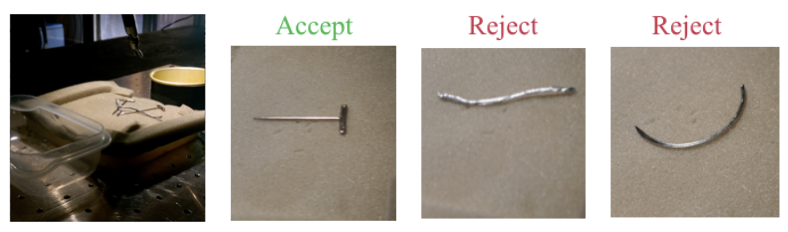
\includegraphics[width=0.58\textwidth]{ddco-experiments/needle-sorting2.png}
    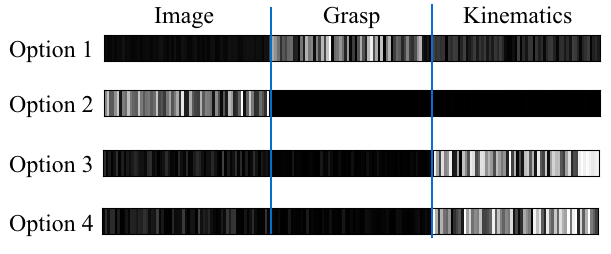
\includegraphics[width=0.4\textwidth]{ddco-experiments/ReLU-dvrk-options.png}
    \caption{(Left) Surgical Bin Picking: the robot is given a foam bin with a pile of 5--8 needles of three different types, each 1--3mm in diameter. The robot must extract needles of a specified type and place them in an ``accept'' cup, while placing all other needles in a ``reject'' cup. (Right) For each of the 4 options, we plot how heavily the different inputs are weighted (\textsf{image}, \textsf{grasp}, or \textsf{kin}) in computing the option's action. Nonzero values of the ReLU units are marked in white and indicate input relevance. \label{fig:dvrkexp4}} 
\end{figure}


We apply \alg to the collected demonstrations with the policy architecture described in \textbf{SM 1.4}. In this network, there are three inputs: a binary \textsf{image}, a candidate \textsf{grasp}, and kinematics (\textsf{kin}). These inputs are processed by distinct branches of the network before being aggregated into a single feature layer.  Using the cross-validation technique described in~\sref{k-validation}, we selected the number of options to be $k=4$.

We plot the average activations of the feature layer for each low-level option (Figure \ref{fig:dvrkexp4}). While this is only a coarse analysis, it gives some indication of which inputs (\textsf{image}, \textsf{grasp}, or \textsf{kin}) are relevant to the policy and termination. We see that the options are clearly specialized. The first option has a strong dependence only on the \textsf{grasp} candidate, the second option attends almost exclusively to the \textsf{image}, while the last two options rely mostly on \textsf{kin}.
The experimental details are described below:
\vspace{0.5em} \noindent \textbf{Task Description: } We consider a task with a more complicated high-level structure.
In this task, the robot is given a foam bin with 3 different types of needles (1mm-3mm in diameter) lying in a pile (5-8 needles in experiments).
The robot must extract a particular type of needle  and place it in the accept cup and place all others in a reject cup.
The task is successful if the entire foam bin is cleared.

Figure \ref{fig:dvrkcats} shows representive objects for this task. We consider three types of ``needles'': dissection pins, suturing needles, and wires.
Dissection pins are placed in the accept cup and the other two are placed in the reject cup.


\vspace{0.5em} \noindent \textbf{Robot and State-Space Parameters: } As in the previous task, the task requires learning because the kinematics of the dvrk are such that the precision needed for grasping needles requires visual servoing.
However, even with visual servoing, failures are common due to the pile (grasps of 2, 3, 4 objects).
We would like to automatically learn recovery behaviors. 
In our robotic setup, there is an overhead endoscopic stereo camera, and it is located 650mm above the workspace.

To define the state-space for this task, we first generate binary images from the stereo images and apply a color-based segmentation to identify the needles (we call this feature \textsf{image}).
Then, we use a classifier derived from 40 hand-labeled images to identify possible grasp points to sample a candidate grasp ( left pixel value, right pixel value, and direction) (we call this feature \textsf{grasp}). 
These features are visualized in Figure \ref{fig:dvrkim}.
Additionally, there is the 6 DoF robot gripper pose and the open-close state of the gripper (we call this feature \textsf{kin}).
The state-space of the robot is (\textsf{kin}, \textsf{image}, \textsf{grasp}), and the action space for the robot is 6 joint angles and the gripper angle.
Each grasp, lift, move, and drop operation consists of 10 time steps of joint angle positions. The motion between the joint angles is performed using a SLURP-based motion planner.



\begin{figure}
    \centering
    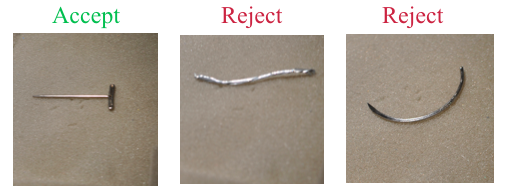
\includegraphics[width=0.6\textwidth]{ddco-experiments/bin-picking-cats.png}
    \caption{There are two bins, one accept and one reject bin. In the accept bin, we place dissection pins and place the suturing needles and the wires in the other. \label{fig:dvrkcats}}
\end{figure}





\vspace{0.5em} \noindent \textbf{Demonstration Protocol: } As in the previous task, to collect demonstrations, we start with a hard-coded open-loop policy.
We roll this policy out and interrupt the policy when we anticipate a failure.
Then, we kinesthetically adjust the pose of the dvrk and it continues.
We collected 60 such demonstrations of fully clearing the bin filled with 3 to 8 needles each--corresponding to 450 individual grasps.
We also introduced a key that allows the robot to stop in place and drop it current grasped needle.
Recovery behaviors were triggered when the robot grasps no objects or more than one object.
Due to the kinesthetic corrections, a very high percentage of the attempted grasps (94\%) grasped at least one object. 
Of the successful grasps, when 5 objects are in the pile 32\% grasps picked up 2 objects, 14\% picked up 3 objects, and 0.5\% picked up 4.
In recovery, the gripper is opened and the epsiode ends leaving the arm in place.
The next grasping trial starts from this point.


\begin{figure} [t]
    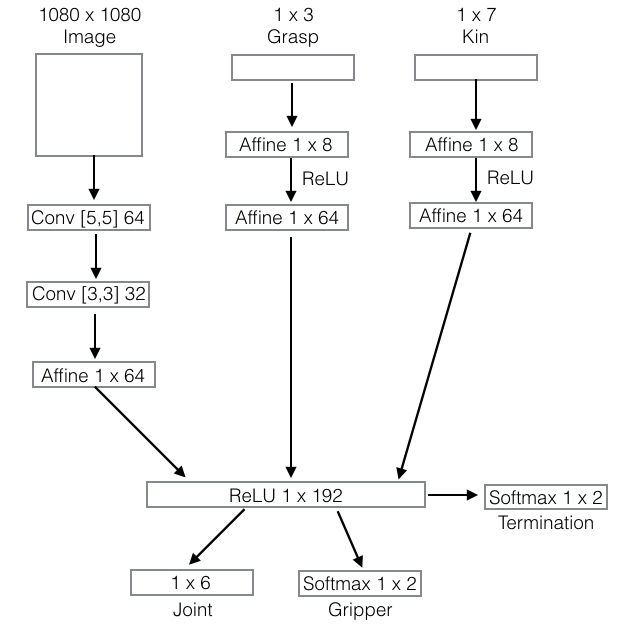
\includegraphics[width=0.48\textwidth]{ddco-experiments/net.png}
    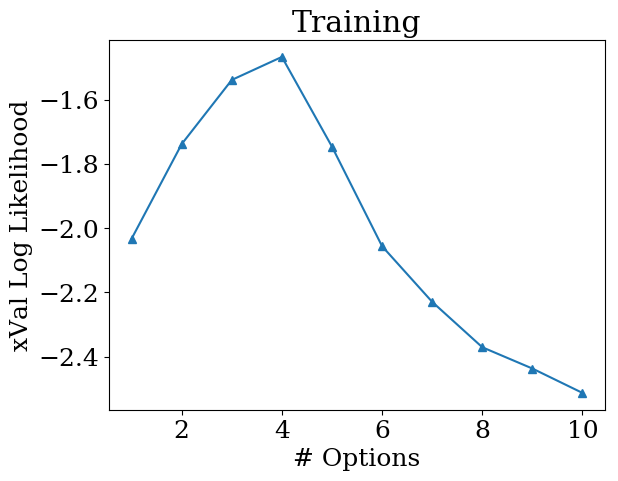
\includegraphics[width=0.48\textwidth]{ddco-experiments/exp6-1.png}
    \caption{We use the above neural network to parametrize each of the four options learned by \alg. In this network, there are three inputs the a binary image, a candidate grasp, and kinematics. These inputs are processed through individual neural net branches and aggregated into a single output layer. This output layer sets the joint angles of the robot and the gripper state (open or closed). Option termination is also determined from this output. \label{fig:dvrknet}}
\end{figure}

\vspace{0.25em} \noindent \textbf{Policy Parametrization: } We apply \alg to the collected demonstrations with the policy parametrization described in Figure \ref{fig:dvrknet}. In this network, there are three inputs the a binary image, a candidate grasp, and kinematics. These inputs are processed through individual neural net branches and aggregated into a single output layer. This output layer sets the joint angles of the robot and the gripper state (open or closed). Option termination is also determined from this output. Using the cross-validation technique described in the paper, we identify 4 options (Figure \ref{fig:dvrknet}). The high-level policy has the same parametrization but after the output layer there is a softmax operation that selects a lower-level option.  

\begin{figure} [t]
    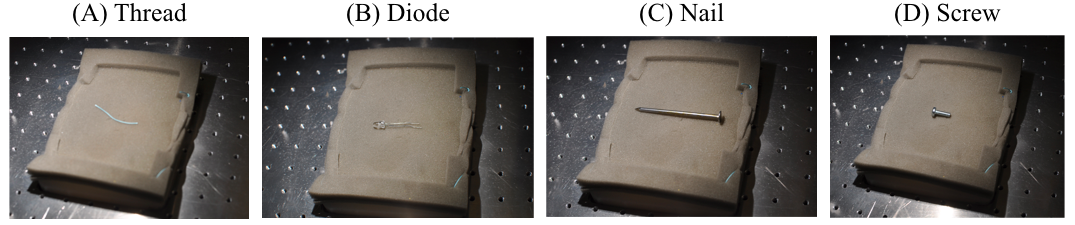
\includegraphics[width=\textwidth]{ddco-experiments/unseen.png}
    \caption{We evaluated the generalization of the learned policy on a small set of unseen objects. This was to understand what features of the object binary mask is used to determine behaviors.\label{fig:dvrkgen}}
\end{figure}

\vspace{0.25em} \noindent \textbf{Coordinate Systems: } We also experimented with different action space representations to see if that had an effect on single object grasps and categorizations. We trained alternative policies with the collected dataset where instead of predicting joint angles, we alternatively predicted 6 DoF end-effector poses with a binary gripper open-close state , and end-effector poses represented a rotation/translation matrix with a binary gripper open-close state. 
We found that the joint angle representation was the most effective. 
In particular, we found that for the grasping part of the task, a policy that controlled the robot in terms of tooltip poses was unreliable.

\begin{table}[ht!]\footnotesize
\centering
\label{my-label}
\begin{tabular}{l|l|l|l|l|}
       & Items & Successful Grasp & Successful Recovery & Successful Categorizations \\
       \hline
Joint Angle & 8     & 7/8         & 2/2    & 7/7                         \\
Tooltip Pose  & 8     & 3/8         & 5/5    & 3/3                             \\
Rotation   & 8     & 2/8          & 0/8    & 0                     
\end{tabular}
\end{table}
\begin{figure} [t]
\centering
    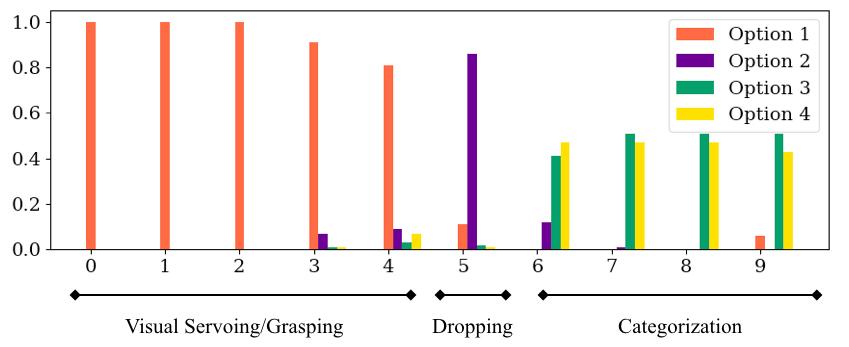
\includegraphics[width=0.8\textwidth]{ddco-experiments/highlevel-options.png}
    \caption{We plot the time distribution of the options selected by the high-level policy. The x-axis represents time, and the bars represent the probability mass assigned to each option. We find that the structure of the option aligns with key phases in the task such as servoing to the needle, grasping it, and categorizing. \label{fig:dvrkhl}}
\end{figure}

\vspace{0.25em} \noindent \textbf{Interpreting Learned Options: }
We additionally analyzed the learned options to see if there was an interpretable structure.
We examined the collected demonstrations and looked at the segmentation structure.
We average over the 60 trials the probability for the high-level policy to choose each option in each of first 10 time-steps during training (Figure \ref{fig:dvrkhl}). We find that the options indeed cluster visited states and segment them in alignment with key phases in the task, such as servoing to the needle, grasping it, dropping it if necessary, and categorizing it into the accept cup. 

\vspace{0.25em} \noindent \textbf{Full Break Down of Experimental Results: }
In 10 trials, 7 out of 10 were successful (Table \ref{big-experiment}). The main failure mode was unsuccessful grasping (defined as either no needles or multiple needles). As the piles were cleared and became sparser, the robot's grasping policy became somewhat brittle. The grasp success rate was 66\% on 99 attempted grasps. In contrast, we rarely observed failures at the other aspects of the task. Of the grasps that failed, nearly 34\% were due to grasping multiple objects.


\begin{table*}[ht!]\footnotesize
\centering
\label{big-experiment}
\begin{tabular}{llllll}
\rowcolor[HTML]{000000} 
{\color[HTML]{FFFFFF} Trial \#} & {\color[HTML]{FFFFFF} \# of Needles} & {\color[HTML]{FFFFFF} \# Needles Cleared} & {\color[HTML]{FFFFFF} Grasping} & {\color[HTML]{FFFFFF} Recovery} & {\color[HTML]{FFFFFF} Categorization} \\
1                               & 6                                    & {\color[HTML]{32CB00} \textbf{6}}         & 6/9                             & 3/3                             & 6/6                                   \\
2                               & 8                                    & 6                                         & 7/12                            & 5/6                             & 6/7                                   \\
3                               & 7                                    & {\color[HTML]{32CB00} \textbf{7}}         & 7/8                             & 1/1                             & 7/7                                   \\
4                               & 6                                    & {\color[HTML]{32CB00} \textbf{6}}         & 6/10                            & 4/4                             & 6/6                                   \\
5                               & 7                                    & 6                                         & 6/11                            & 5/5                             & 6/6                                   \\
6                               & 8                                    & {\color[HTML]{32CB00} \textbf{8}}         & 8/13                            & 5/5                             & 8/8                                   \\
7                               & 6                                    & 5                                         & 5/9                             & 4/4                             & 5/5                                   \\
8                               & 7                                    & {\color[HTML]{32CB00} \textbf{7}}         & 7/10                            & 3/3                             & 7/7                                   \\
9                               & 8                                    & {\color[HTML]{32CB00} \textbf{8}}         & 8/10                            & 2/2                             & 8/8                                   \\
10                              & 6                                    & {\color[HTML]{32CB00} \textbf{6}}         & 6/7                             & 1/1                             & 6/6                                   \\
Totals                          & 69                                   & Success: 70\%                             & Success: 66\%                   & Success: 97\%                   & Success: 98\%                        
\end{tabular}
\end{table*}



\vspace{0.25em} \noindent \textbf{Generalization to unseen objects: } We also evaluated the learned policy on a few unseen objects (but similarly sized and colored) to show that there is some level of generalization in the learning. We tried out four novel objects and evaluated what the learned policy did for each (Figure \ref{fig:dvrkgen}). For each of the novel objects we tried out 10 grasps in random locations and orientations in the bin (without any others). We evaluated the grasp success and whether it was categorized consistently (i.e., does the learned policy consistently think it is a pin or a needle).

We found that the diode was consistently grasped and categorized as a dissection pin. We conjecture this is because of its head and thin metallic wires. On the other hand, the screw and the thread were categorized in the reject cup. For 8/10 of the successful grasps, the nail was categorized as a failure mode. We conjucuture that since it is the large object it looks similar to the two object grasps seen in the demonstrations.

% Please add the following required packages to your document preamble:
% \usepackage[normalem]{ulem}
% \useunder{\uline}{\ul}{}
\begin{table}[ht!]\footnotesize
\centering
\label{my-label}
\begin{tabular}{l|l|l|l|l|l}
       & Grasps & Successful & Drop & Categorize Accept & Categorize Reject \\
       \hline
Thread & 10     & 10         & 1    & 0              & 9                 \\
Diode  & 10     & 10         & 0    & 10             & 0                 \\
Nail   & 10     & 8          & 8    & 0              & 0                 \\
Screw  & 10     & 4          & 0    & 0              & 4                
\end{tabular}
\end{table}


Finally, we evaluate the success of the learned hierarchical policy in 10 full trials, according to 4 different success criteria. First, the overall task success is measured by the success rate of fully clearing the bin without failing 4 consecutive grasping attempts. Second, we measure the success rate of picking exactly one needle in individual grasp attempts. Third, we measure the success rate of appropriately reacting to grasps, by dropping the load and retrying unsuccessful grasps, and not dropping successful grasps. Fourth, we measured the success rate of needle categorization.

In 10 trials, 7/10 were successful. The main failure mode was unsuccessful grasping due to picking either no needles or multiple needles. As the piles were cleared and became sparser, the robot's grasping policy became somewhat brittle. The grasp success rate was 66\% on 99 attempted grasps. In contrast, we rarely observed failures at the other aspects of the task, reaching 97\% successful recovery on 34 failed grasps. The Supplementary Material (\textbf{SM 1.4}) describes a full breakdown of the failure modes, as well as an additional experiment of policy generalization to unseen objects.


\subsubsection{Vector Quantization For Initialization}
One challenge with \alg is initialization.
When real perceptual data is used, if all of the low-level policies initialize randomly the forward-backward estimates needed for the Expectation-Gradient will be poorly conditioned where there is an extremely low likelihood assigned to any particular observation.
The EG algorithm relies on a segment-cluster-imitate loop, where initial policy guesses are used to segment the data based on which policy best explains the given time-step, then the segments are clustered, and the policies are updated.
In a continuous control space, a randomly initialized policy may not explain any of the observed data well.
This means the small differences in initialization can lead to large changes in the learned hierarchy.

We found that a necessary pre-processing step was a variant of vector quantization, originally proposed for problems in speech recognition. 
We first cluster the state observations using a \textsf{k-means} clustering and train $k$ behavioral cloning policies for each of the clusters.
We use these $k$ policies as the initialization for the EG iterations.
Unlike the random initialization, this means that the initial low level policies will demonstrate some preference for actions in different parts of the state-space.
We set $k$ to be the same as the $k$ set for the number of options, and use the same optimization parameters.

\subsubsection{Layer-wise Hierarchy Training}
We also found that layer-wise training of the hierarchy greatly reduced the likelihood of a degenerate solution.
While, at least in principle, one can train 
When the meta-policy is very expressive and the options are initialized poorly, sometimes the learned solution can degenerate to excessively using the meta-policy (high-fitting). 
We can avoid this problem by using a simplified parametrization for the meta-control policy $\eta_d$ used when discovering the low-level options. For example, we can fix a uniform meta-control policy that chooses each option with probability $\nicefrac 1 {k}$. Now, once these low-level options are discovered, then we can augment the action space with the options and train the meta-policy.

This same algorithm can recursively proceed to deep hierarchies from the lowest level upward: level-$d$ options can invoke already-discovered lower-level options; and are discovered in the context of a simplified level-$d$ meta-control policy, decoupled from higher-level complexity.
Perhaps counter-intuitively, this layer-wise training does not sacrifice too much during option discovery, and in fact, initial results seem to indicate that it improves the stability of the algorithm.
An informative meta-control policy would serve as a prior on the assignment of demonstration segments to the options that generated them, but with sufficient data this assignment can also be inferred from the low-level model, purely based on the likelihood of each segment to be generated by each option.


\begin{figure} [t]
\centering
    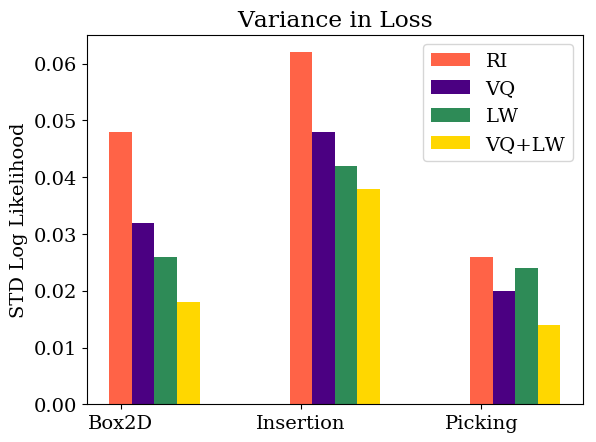
\includegraphics[width=0.3\textwidth]{ddco-experiments/exp8-1.png}
    \caption{This experiment measures the variance in log likelihood over 10 different runs of \alg with different training and initialization strategies. Vector Quantization (VQ) and Layer-Wise training (LW) help stabilize the solution. \label{fig:exp81}}
\end{figure}

\begin{figure} [t]
\centering
    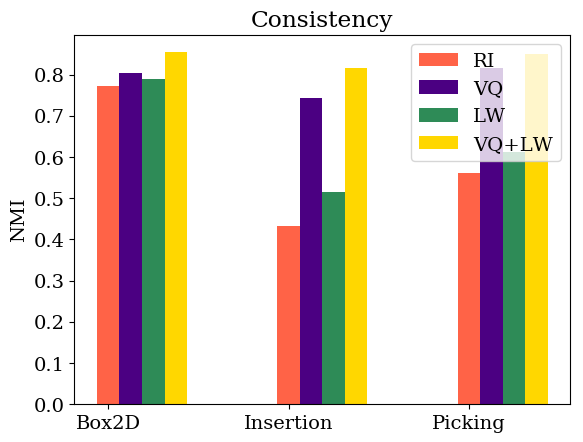
\includegraphics[width=0.3\textwidth]{ddco-experiments/exp8-2.png}
    \caption{We measure the average normalized mutual information between multiple runs of \alg. This measures the consistency of the solutions across intializations. \label{fig:exp82}}
\end{figure}


\begin{figure} [t]
\centering
    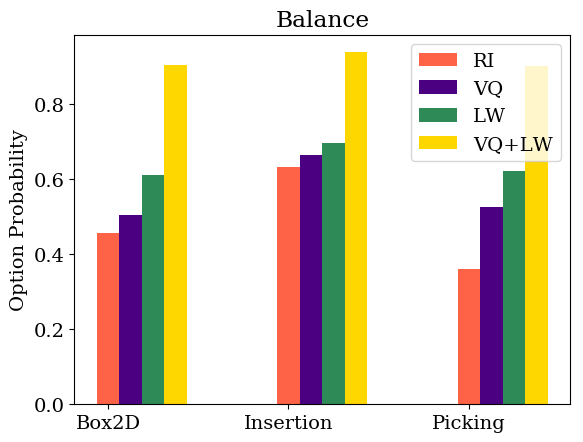
\includegraphics[width=0.3\textwidth]{ddco-experiments/exp8-3.png}
    \caption{We measure probability that an option is selected by the high-level policy. \label{fig:exp83}}
\end{figure}

\subsubsection{Results: Stability of \alg}
In the first experiment, we measure the variance in log likelihood over 10 different runs of \alg with different training and initialization strategies (Figure \ref{fig:exp81}). 
We use the entire datasets presented in the paper and use the FF architecture for the Box2D experiments.
Vector Quantization (VQ) and Layer-Wise training (LW) help stabilize the solution and greatly reduce the variance of the algorithm.
This reduction in variance is over 50\% in the Box2D experiments, and a little more modest for the real data.

In the next experiment, we measure the consistency of the solutions found by \alg (Figure \ref{fig:exp82}).
For each of the demonstration trajectories, we annotate the time-step by the most likely option.
One can view this annotation as a hard clustering of the state-action tuples.
Then, we measure the average normalized mutual information (NMI) between all pairs of the 10 different runs of \alg.
NMI is a measure of how aligned two clusterings are between 0 and 1, where 1 indicates perfect alignment.
As with the likelihood, Vector Quantization (VQ) and Layer-Wise training (LW) significantly improve the consistency of the algorithm.


In the last experiment, we measure the symptoms of the ``high-fitting'' problem (Figure \ref{fig:exp83}).
We plot the probability that the high-level policy selects an option.
In some sense, this measures how much control the high-level policy delegates to the options.
Surprisingly, VQ and LW have an impact on this.
Hierarchies trained with VQ and LW have a greater reliance on the options.

\begin{figure} [t]
\centering
    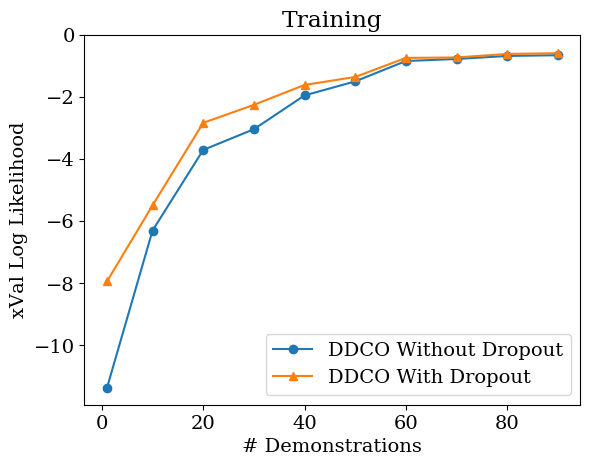
\includegraphics[width=0.4\textwidth]{ddco-experiments/exp9.png}
    \caption{Dropout seems to have a substantial effect on improving cross-validation accuracy on a hold out set. \label{fig:exp9}}
\end{figure}

\subsubsection{The Effects of Dropout}
For the real datasets, we leverage a technique called dropout, which has been widely used in neural network training to prevent overfitting.
Dropout is a technique that randomly removes a unit from
the network along with all its connections.
We found that this technique improved performance when the datasets were small. We set the dropout parameter to 0.5 and measured the performance on a hold out set.
We ran an experiment on the needle insertion task dataset, where we measured the cross-validation accuracy on held out data with and without dropout (Figure \ref{fig:exp9}).
Dropout seems to have a substantial effect on improving cross-validation accuracy on a hold out set.

\subsection{Experiments: Reinforcement}
We present an empirical study of \alg in the Reinforcement Learning setting. Our results suggest that \alg can discover options that accelerates reinforcement learning.
We explore two different scenarios: (\textbf{Supervised}) given a supervisor who demonstrates a few times how to perform a task, show that the discovered options are useful for accelerating reinforcement learning on the same task; (\textbf{Exploration}) apply reinforcement learning for $T$ episodes, sample trajectories from the current best policy, and augment the action space with the discovered options for the remaining $T'$ episodes. 
The first set of experiments illustrates \alg on a series of GridWorld domains.
Then, we show how the Expectation-Gradient can scale to more challenging Atari RAM domains.
Finally, we show that \alg can be used to identify visuomotor primitives in surgical data.

\begin{figure}[t]
    \centering
    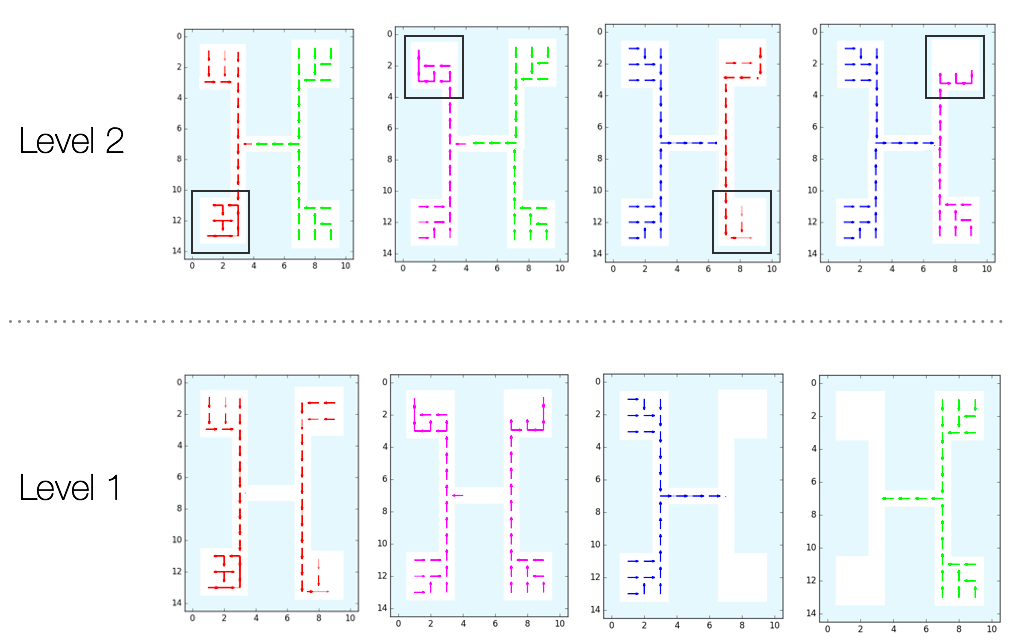
\includegraphics[width=\columnwidth]{ddco-experiments/ddo-4-rooms-results.png}
    \caption{Trajectories generated by options in a hierarchy discovered by \alg. Each level has 4 options, where level 2 builds on the level 1, which in turn uses atomic actions. In the lower level, two of the options move the agent between the upper and lower rooms, while the other two options move it from one side to the other. 
    In the higher level, each option takes the agent to a specific room. The lower-level options are color-coded to show how they are composed into the higher-level options. \label{gw-1}} 
\end{figure}

\subsubsection{Four Rooms GridWorld \label{exp:gw-four-rooms}}
We study a simple four-room domain~(Figure~\ref{gw-1}). On a $15\times11$ grid, the agent can move in four directions; moving into a wall has no effect. To simulate environment noise, we replace the agent's action with a random one with probability $0.3$. An observable apple is spawned in a random location in one of the rooms. Upon taking the apple, the agent gets a unit reward and the apple is re-spawned.

\begin{figure}[t]
    \centering
    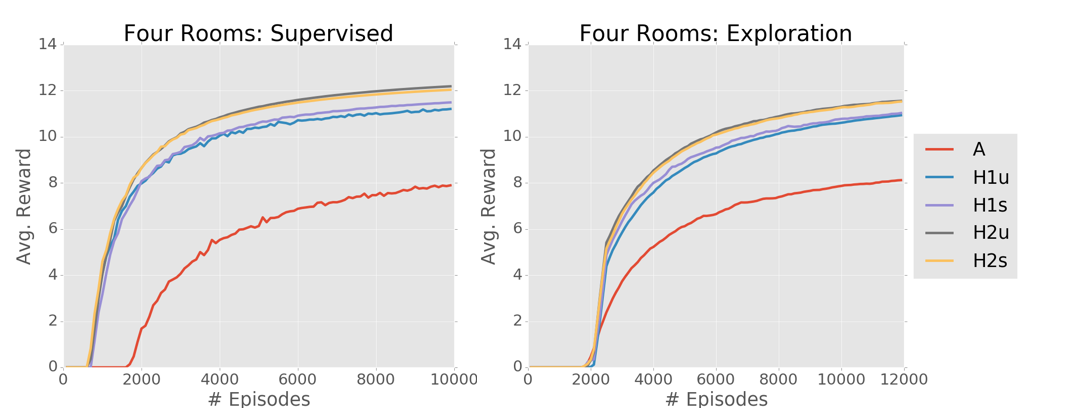
\includegraphics[width=\columnwidth]{ddco-experiments/4-rooms-clean.png}
    \caption{$15$-trial mean reward for the Supervised and Exploration problem settings when running DQN with no options (\textsf{A}), low-level options (\textsf{H1u}) and lower- and higher-level options (\textsf{H2u}) augmenting the action space. The options discovered by \alg can accelerate learning, since they benefit from not being interrupted by random exploration.  \label{gw-2}}
\end{figure}

We use the following notation to describe the different ways we can parametrize option discovery: \textsf{A} a baseline of only using atomic actions; \textsf{H1u} discovering a single level of options where the higher-level is parametrized by a uniform distribution; \textsf{H1s} discovering a single level of options where the higher-level is parametrized by an multi-layer perceptron (MLP); \textsf{H2u} and \textsf{H2s} are the two-level counterparts of \textsf{H1u} and \textsf{H1s}, respectively. All of these discovered options are used in an RL phase to augment the action space of a high-level global policy.

\begin{figure*}[ht]\vspace{-1em}
    \centering
    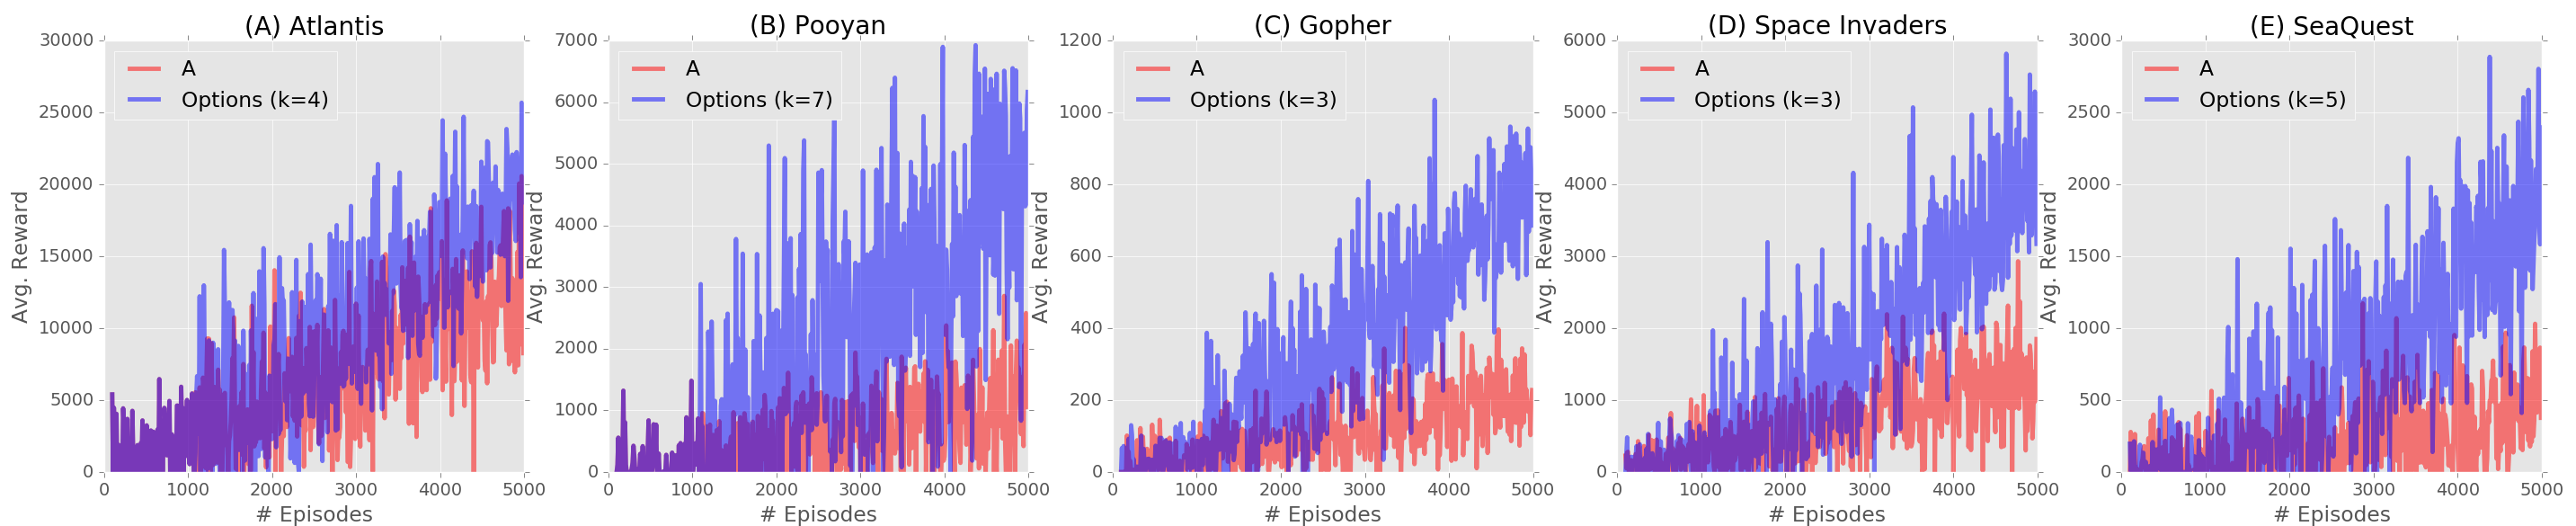
\includegraphics[width=\textwidth]{ddco-experiments/exp5-atari.png}
    \caption{Atari RAM Games: Average reward computed from 50 rollouts when running DQN with atomic actions for 1000 episodes, then generating 100 trajectories from greedy policy, from which \alg discovers options in a 2-level hierarchy. DQN is restarted with action space augmented by these options, which accelerates learning in comparison to running DQN with atomic actions for 5000 episodes. Results suggest significant improvements in 4 out of 5 domains. \label{atari-1}}\vspace{-1em}
\end{figure*}

{\bf Supervised Setting.} We use Value Iteration to compute the optimal policy, and then use this policy as a supervisor to generate 50 trajectories of length 1000. All policies, whether for control, meta-control or termination, are parametrized by a MLP, with a single two-node hidden layer, and $\tanh$ activation functions. The MLP's input consists of the full state (agent and apple locations), and the output is computed by a $\mathrm{softmax}$ function over the MLP output vector, which has length $|\C A|$ for control policies and two for termination.

The options corresponding to \textsf{H2u} are visualized in Figure~\ref{gw-1} by trajectories generated using each option from a random initial state until termination. At the first level, two of the discovered options move the agent between the upper and lower rooms, and two move it from one side to the other. At the second level, the discovered options aggregate these primitives into higher-level behaviors that move the agent from any initial location to a specific room.

{\bf Impact of options and hierarchy depth.} To evaluate the quality of the discovered options, we train a Deep Q-Network (DQN) with the same MLP architecture, and action space augmented by the options. The exploration is $\epsilon$-greedy with $\epsilon=0.2$ and the discount factor is $\gamma=0.9$. Figure~\ref{gw-2} shows the average reward in $15$ of the algorithm's runs in the Supervised and Exploration experimental settings.
The results illustrate that augmenting the action space with options can significantly accelerate learning. Note that the  options learned with a two-level hierarchy (\textsf{H2u}) provide significant benefits over the options learned only with a single-level hierarchy \textsf{H1u}.
The hierarchical approaches achieve roughly the same average reward after 1000 episodes as \textsf{A} does after 5000 episodes.

{\bf Impact of policy parametrization.} To evaluate the effect of meta-control policy parametrization, we also compare the rewards during DQN reinforcement learning with options discovered with MLP meta-control policies (\textsf{H1s} and \textsf{H2s}). Our empirical results suggest that less expressive parametrization of the meta-control policy does not significantly hurt the performance, and in some cases can even provide a benefit (Figure \ref{gw-2}). This is highly important, because the high sample complexity of jointly training all levels of a deep hierarchy necessitates simplifying the meta-control policy --- which would otherwise be represented by a one level shallower hierarchy. We conjecture that the reason for the improved performance of the less expressive model is that more complex parametrization of the meta-control policy increases the prevalence of local optima in the inference problem, which may lead to worse options.

{\bf Exploration Setting.} Finally, we demonstrate that options can also be useful when discovered from self-demonstrations by a partially trained agent, rather than by an expert supervisor. We run the same DQN as above, with only atomic actions, for 2000 episodes. We then use the greedy policy for the learned $Q$-function to generate 100 trajectories.  We reset the $Q$-function (except for the baseline \textsf{A}), and run DQN again with the augmented action space. Figure \ref{gw-2} illustrates that even when these options are not discovered from demonstrations of optimal behavior, they are useful in accelerating reinforcement learning.
The reason is that options are policy fragments that have been discovered to lead to interesting states, and therefore benefit from not being interrupted by random exploration. 

%\ion{This paragraph is confusing. Not sure what does "30\% probability of random action" exactly mean. Not sure where the 11 goals are coming from.}In the first scenario, we construct a 15x10 GridWorld environment with four rooms with a 30\% probability of random action. Goal states are randomly drawn in each room and the agent has accumulate as many goals as possible in 1000 timesteps or a maximum of 11 total goals (each goal results in a reward of 1). We generate 50 demonstrations using Value Iteration. 

%\vspace{0.25em} \noindent \textbf{Model Parameterization: } The agent's state is a 4-dimensional vector $(x,y, g_x, g_y)$ where $(g_x,g_y)$ is the current goal. \ion{What does {\bf current} goal mean?} For this experiment, each  low-level option is a multi-layer perceptron (MLP) with a single hidden layer consisting of $2$ nodes that employ $\textsf{tanh}$ activation functions. The high-level meta-policy is parameterized by an i.i.d  uniform distribution. One of our hypotheses is that in the option discovery phase simple high-level policies suffice, as these policies will ultimately be re-learned on the transfer instance.

%\vspace{0.25em} \noindent \textbf{Learned Hierarchy: } We apply \alg to learn a two-level hierarchy where each level has four options (Figure \ref{gw-1}). The visualization shows trajectories sampled from the inferred options, i.e., start at a random state and apply the option until termination. Out of the four options we discover at the low level, two move the agent from the upper two rooms to the lower two rooms, and two move the agent from one side to the other. By adding a second level to the hierarchy \Roy{so this is L2+L3 after L1+U?}, we get higher level behaviors by aggregating the low-level options. In particular, the options we discover at the second level move an agent to a {\em particular} room starting from a random location.

%\vspace{0.25em} \noindent \textbf{Evaluating the Options: } Consider a new task instance where goal states are randomly sampled. Next, we evaluate whether (and how much) the options we learned in the two-level hierarchy improve the convergence of an RL algorithm. We use a Deep Q Network (DQN) as the RL algorithm. The Q-Network uses the same architecture as the options, i.e., a single-hidden layer MLP with two hidden nodes. We train the network with an $\epsilon$-greedy policy with discount factor of $\gamma=0.9$, and $\epsilon=0.2$, respectively.
%We compare three approaches: (1) DQN using only primitive actions, (2) DQN using the low-level options, in additions to all primitive actions, and (3) DQN using the options at both levels of the hierarchy, as well as all primitive actions.
%Figure \ref{gw-2} shows the average reward for each approach versus the number of episodes. These results clearly illustrate that augmenting the action space with options can significantly improve the convergence. There are two points worth noting. First, approach 3 (i.e., leveraging all options and primitive actions) achieves the same average reward as approach 1, 5x faster. Indeed, after less than $1000$ episodes, approach 3 achieves roughly the same average reward as approach 1 after $5000$ episodes. Second, the deeper hierarchy provides significant benefits over the single-level hierarchy. This is because options allow the agent to receive a reward faster.



%\vspace{0.25em} \noindent \textbf{Evaluating the Parameterization: } Next, we evaluate different parameterization strategies for the \alg. In particular, we consider the impact of the high-level meta policy's parameterization during the learning stag. In particular, we consider the following variants of the two-level hierarchy described before: (\textsf{L0}) No options, (\textsf{L1u}) single level of options with a uniform meta policy, (\textsf{L2u}) two levels of options both learned with uniform meta policies, (\textsf{L1s}) a single level of options learned with a state-dependent MLP meta policy, and (\textsf{L2s}) two levels of options both learned with state-dependent MLP meta policies. Using a uniform meta policy during the inference stage significantly reduces the number of parameters for learning, and our experimental results suggest that such a parameterization does not significantly hurt the performance (Figure \ref{gw-3}). In fact, results suggest that in some cases, the additional parameters can actually hurt. We conjecture this is because the more complex parameterization of the meta policies increases the number of local minima in the inference problem, which ultimately leads to some lower quality options.

%The decoupling between the low-level options and the high-level meta-policy is interesting because it facilitates scaling the hierarchy. If each level is decoupled from the previous one, it is easy to scale the number of levels in the hierarchy. Furthermore, the reduced parameterization improves learning performance (i.e., requires fewer demonstrations). However, we must caution that this is not a definitive result and warrants further investigating, which we plan to do in future work. There are clearly situations where using a more complex parameterization of the high-level policy can help differentiate between equally likely option assignments. Nonetheless, next, we leverage these preliminary results as a motivation for using a simplified high-level structure during the option discovery phase. 


%\subsection{GridWorld: Incremental}
%The previous scenario illustrates how options can facilitate transfer between task instances. Next, we show how within a task options can be used to improve the convergence of an RL algorithm by incrementally constructing options.
%We use the same four-room GridWorld as before.
%We use a Deep Q Network (DQN) as the RL algorithm.
%The Q-Network is constructed with the same basic architecture as the options (single-hidden layer MLP, 2 hidden nodes), and we train the network with an $\epsilon$-greedy policy with discount factor of $\gamma=0.9$ and $\epsilon=0.2$.
%We run the DQN over the original primitive action space for $2000$ episodes, then sample $100$ demonstrations from the current best policy, and then apply \alg. The future $13000$ episodes of the DQN are run with an augmented action space.
%This DQN is re-initialized and trained from scratch. 
%Figure \ref{gw-4} illustrates that even when these options are not derived from an optimal supervisor, they are useful in improving the long term performance of the agent.
%This is because that the agent is allowed to reuse previously learned behaviors without having to re-learn them through exploration.


\subsubsection{Atari RAM Games}
The RAM variant of the popular Atari Deep Reinforcement Learning domains considers a game-playing agent which is given not the screen, but rather the RAM state of the Atari machine.
This RAM state is a 128-byte vector that completely determines the state of the game, and can be encoded in one-hot representation as $s\in\F R^{128 \times 256}$.
The RAM state-space illustrates the power of an automated option discovery framework, as it would be infeasible to manually code options without carefully understanding the game's memory structure.
With a discovery algorithm, we have a general-purpose approach to learn in this environment.

All policies are parametrized with a deep network. There are three dense layers, each with $\tanh$ activations, and the output distribution is a $\mathrm{softmax}$ of the last layer, which has length $|\C A|$ for control policies and two for termination. We use a single level of options, with the number of options tuned to optimize performance, and given in Figure~\ref{atari-1}.

For each game, we first run the DQN for $1000$ episodes, and then generate $100$ trajectories from the greedy policy, and use them to discover options with \alg.
The DQN has the same architecture, using $\epsilon$-greedy exploration for $1000$ episodes with $\epsilon=0.05$ and discount factor $\gamma=0.85$ (similar to the parameters used in~\citep{sygnowski2016learning}). 
Finally, we augment the action space with the discovered options and rerun DQN for $4000$ episodes. 
We compare this to the baseline of running DQN for $5000$ episodes with actions only.

Figure \ref{atari-1} plots the estimate value, averaged over $50$ trials, of the learned policies for five Atari games: Atlantis, Pooyan, Gopher, Space Invaders, and Sea Quest.
In four out of five games, we see a significant acceleration learning.
The relative improvements are the largest for the three hardest domains: Gopher, Sea Quest, and Space Invaders.
It is promising that \alg offers such an advantage where other methods struggle. 
Figure \ref{atari-3} shows four frames from one of the options discovered by \alg for the Atlantis game. %\footnote{In the final version, we will provide a link to the videos of the learned options.}.
The option appears to identify an incoming alien and determine when to fire the gun, terminating when the alien is destroyed.
As in the GridWorld experiments, the options are policy fragments that have been discovered to lead to high-value states, and therefore benefit from not being interrupted by random exploration.

\begin{figure}[t]\vspace{-1em}
    \centering
    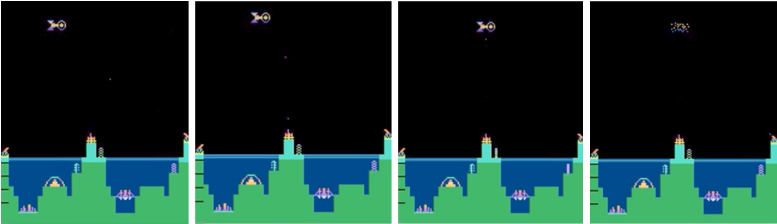
\includegraphics[width=\columnwidth]{ddco-experiments/atlantis-primitive.png}
    \caption{Frames sampled from a demonstration trajectory assigned to one of the primitives learned from \alg.  \label{atari-3}}
\end{figure}

\subsubsection{Segmentation of Robotic-Assisted Surgery}
In this section, we illustrate the wide applicability of the \alg framework by applying it to human demonstrations in a robotic domain. We apply \alg to long robotic trajectories (e.g. 3 minutes) demonstrating an intricate task, and discover options for useful subtasks, as well as segmentation of the demonstrations into semantic units.
The JIGSAWS dataset consists of surgical robot trajectories of human surgeons performing training procedures~\citep{gao2014jigsaws}. 
The dataset was captured using the da Vinci Surgical System from eight surgeons with different skill levels, performing five repetitions each of \emph{needle passing}, \emph{suturing}, and \emph{knot tying}.
This dataset consists of videos and kinematic data of the robot arms, and is annotated by experts identifying the activity occurring in each frame.

Each policy network takes as input a three-channel RGB $200 \times 200$ image, downscaled from $640 \times 480$ in the dataset, applies three convolutional layers with ReLU activations followed by two fully-connected dense layers reducing to $64$ and then eight real-valued components. An action is represented by 3D translations and the opening angles of the left and right arm grippers.

We investigate how well the segmentation provided by \alg corresponds to expert annotations, when applied to demonstrations of the three surgical tasks. Figure \ref{surgery-1} shows a representative sample of $10$ trajectories from each task, with each time step colored by the most likely option to be active at that time. Human boundary annotations are marked in $\times$. We quantify the match between the manual and automatic annotation by the fraction of option boundaries that have exactly one human annotation in a $300$ ms window around them. By this metric, \alg obtains $72$\% accuracy, while random guessing gets only $14$\%. These results suggest that \alg succeeds in learning some latent structure of the task.

\begin{figure}[t]
    \centering
    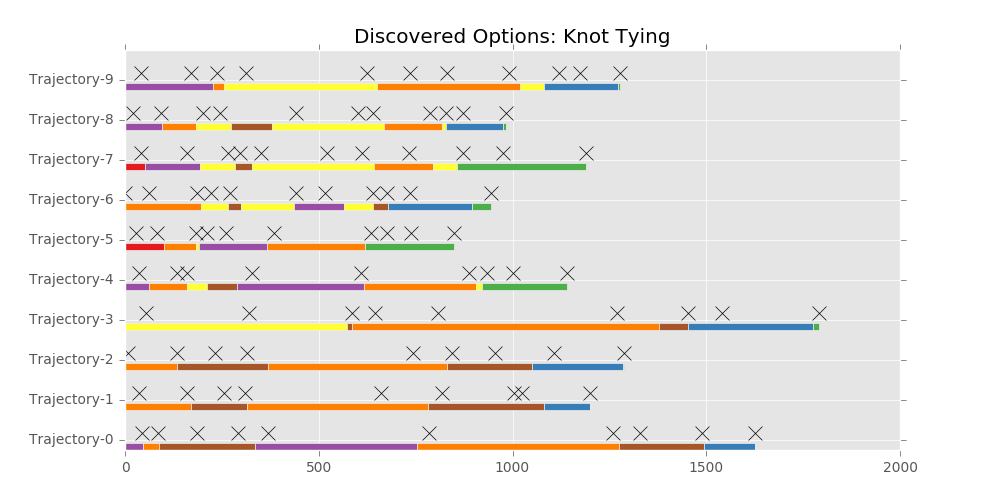
\includegraphics[width=\columnwidth]{ddco-experiments/options-knot-tying.png}
    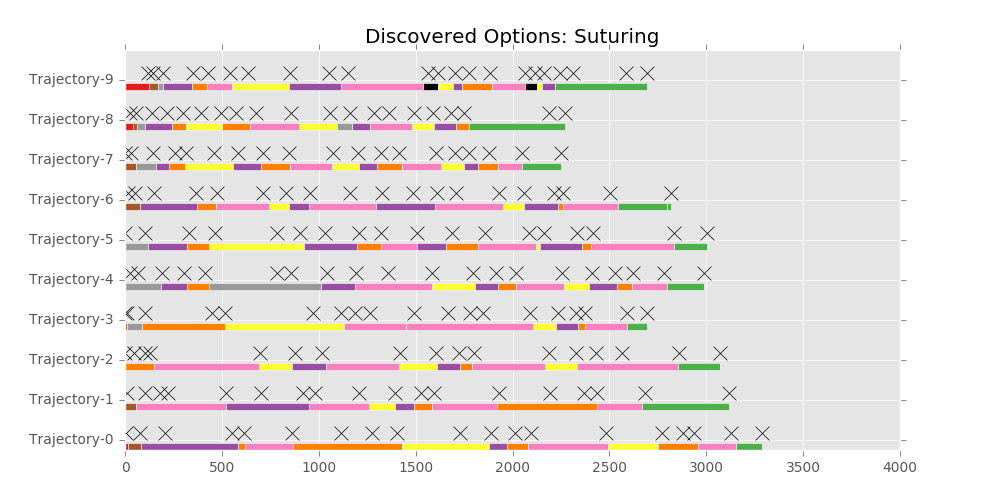
\includegraphics[width=\columnwidth]{ddco-experiments/options-suturing.png}
    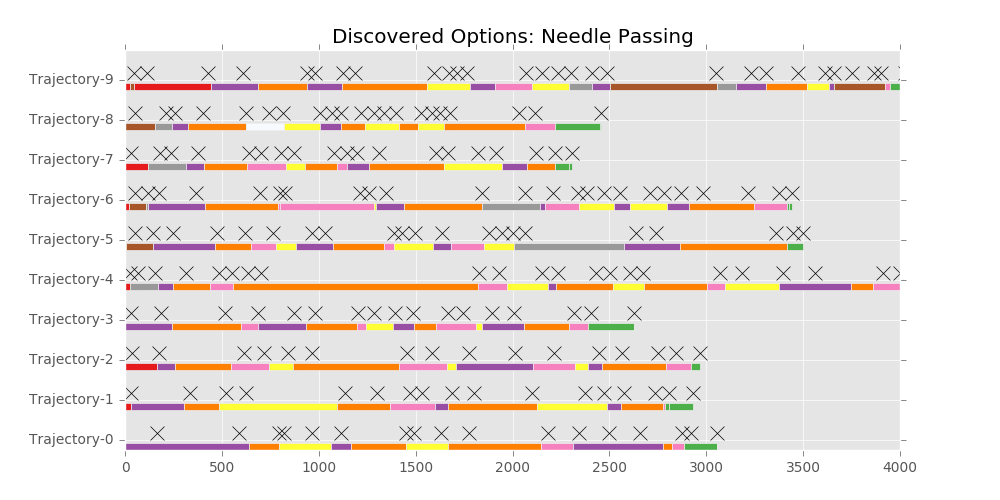
\includegraphics[width=\columnwidth]{ddco-experiments/options-needle-passing.png}
    \caption{Segmentation of human demonstrations in three surgical tasks. Each line represents a trajectory, with segment color indicating the option inferred by \alg as most likely to be active at that time. Human annotations are marked as $\times$ above the segments. Automated segmentation achieves a good alignment with human annotation --- 72\% of option boundaries have exactly one annotation in a 300 ms window around them. \label{surgery-1}}\vspace{-1em}
\end{figure}
